\documentclass[cs4size, a4paper, twoside]{ctexart}
\usepackage{xeCJK}

%章节总标题加点
\usepackage[subfigure]{tocloft}	
\renewcommand{\cftsecleader}{\cftdotfill{\cftdotsep}}  

%==================== 数学符号公式 ============
\usepackage{amsmath}                 % AMS LaTeX宏包
\usepackage{amssymb}                % 用来排版漂亮的数学公式 罗马数字、希腊字母
%\usepackage{amsbsy}
\usepackage[style=1]{mdframed}
\usepackage{amsthm}
\usepackage{amsfonts}
\usepackage{mathrsfs}                % 英文花体字体
\usepackage{bm}                      % 数学公式中的黑斜体
\usepackage{bbding,manfnt}           % 一些图标,如 \dbend
\usepackage{lettrine}                % 首字下沉,命令\lettrine
\def\attention{\lettrine[lines=2,lraise=0,nindent=0em]{\large\textdbend\hspace{1mm}}{}}
\usepackage{longtable}
\usepackage[toc,page]{appendix}
\usepackage{geometry}                % 页边距调整
\geometry{top=3.0cm,bottom=2.7cm,left=2.5cm,right=2.5cm}
%\usepackage{caption2}               % 浮动图形和表格标题样式
\usepackage{siunitx}                 % 温度
\usepackage{mhchem}                  % 化学元素
%====================按章编号==========================
\numberwithin{equation}{section}
\numberwithin{table}{section}
\numberwithin{figure}{section}

%================= 基本格式预置 ===========================
\linespread{1.25} \zihao{-4}  % 行距、字号
\setlength{\parskip}{0pt}  % 段距

% 页眉页脚
\usepackage{fancyhdr}
\pagestyle{fancy}
\fancyhf{}
\fancyhead[OC]{\zihao{5}  \leftmark}
\fancyhead[EC]{\zihao{5} \songti 西安石油大学大学本科毕业设计(论文)}
\fancyfoot[C]{~\zihao{5} —\hspace{0.5em} \thepage \hspace{0.5em}—~}
\renewcommand{\sectionmark}[1]{\markboth{#1}{}}
\renewcommand{\headrulewidth}{0.65pt}

% 标题格式
\CTEXsetup[format={\centering\zihao{-3}\bfseries},beforeskip={1em},afterskip={2em}]{section}
\CTEXsetup[format={\bfseries\zihao{4}},beforeskip={0.5em},afterskip={0.5em}]{subsection}
\CTEXsetup[format={\bfseries\zihao{-4}},beforeskip={0.5em},afterskip={0.5em}]{subsubsection}

% 上标引用格式
\newcommand{\upcite}[1]{\textsuperscript{\textsuperscript{\cite{#1}}}}  
\renewcommand{\cftsecleader}{\cftdotfill{\cftdotsep}}
\usepackage[font=small,labelfont=bf, textfont=bf]{caption}

% 目录不加粗
%\usepackage{tocstyle}
%\usepackage{microtype}
%\settocfeature[toc][1]{entryhook}{\normalfont}


%================== 图形支持宏包 =========================
\usepackage{subfigure}
\usepackage{graphicx}                % 嵌入png图像
\usepackage{color,xcolor}            % 支持彩色文本、底色、文本框等
\usepackage{pifont}                  % 支持圈数字 %\ding{number}
\usepackage{hyperref}                % 交叉引用
\usepackage{caption}
\usepackage{float}
\captionsetup{figurewithin=section}

%==================== 源码和流程图 ====================
\usepackage{listings}                % 粘贴源代码
\lstset{ 
	language=Python,
	tabsize=4, 
	basicstyle=\normalsize\linespread{1.1}\footnotesize\ttfamily,
	showstringspaces=false,
	frame=top, frame=bottom,
	commentstyle=\color{green}, 
	keywordstyle=\color{blue}, 
	breaklines=true,
	numbers=left, numberstyle=\tiny,
}
\usepackage{tikz}                    
\usepackage{tikz-3dplot}
\usetikzlibrary{shapes,arrows,positioning}

%==================== 字体设置 ====================
% Mac 字体设置
%\setCJKmainfont[BoldFont=宋体-简 粗体,ItalicFont=宋体-简 常规体]{宋体-简 常规体}
%\setCJKsansfont[BoldFont=宋体-简 常规体]{宋体-简 常规体}
%\setCJKmonofont{宋体-简 常规体}

\setmainfont{Times New Roman} 
\setCJKmainfont[BoldFont=华文中宋]{宋体}

%==================== 自定义包 =======================

%===================  定理类环境定义 ===================
\newtheorem{example}{例}              % 整体编号
\newtheorem{algorithm}{算法}
\newtheorem{theorem}{定理}            % 按 section 编号
\newtheorem{definition}{定义}
\newtheorem{axiom}{公理}
\newtheorem{property}{性质}
\newtheorem{proposition}{命题}
\newtheorem{lemma}{引理}
\newtheorem{corollary}{推论}
\newtheorem{remark}{注解}
\newtheorem{condition}{条件}
\newtheorem{conclusion}{结论}
\newtheorem{assumption}{假设}
\usepackage{enumitem}


%===================   正文开始   ===================

\begin{document}
	
	%==================重定义 ===================
	\renewcommand{\contentsname}{\hspace*{\fill}目\quad 录\hspace*{\fill}\\}   
	\renewcommand{\abstractname}{摘要} 
	\renewcommand{\refname}{参考文献}     
	\renewcommand{\indexname}{索引}
	\renewcommand\thefigure{\thesection-\arabic{figure}}
	\renewcommand{\figurename}{图}
	\renewcommand\thetable{\thesection-\arabic{table}}
	\renewcommand{\tablename}{表}
	\renewcommand{\appendixname}{附录}
	\renewcommand{\proofname}{证明}
	\renewcommand{\algorithm}{算法} 
	%\renewcommand{\labelenumi}{(\arabic{enumi})}

	% 封皮和前言
	%===============  封面  =================
\smallskip
\vspace*{2.0cm}
\begin{center}
\begin{figure}[!th]
\centering
\includegraphics[width=0.3\linewidth]{figure/SchoolName}
\end{figure}

\vspace*{1.0cm}{\zihao{-1} \textbf{\songti{} 本科毕业设计(论文)}} \\
\vspace*{7.0cm} \songti{}
% 创建表内换行
\newcommand{\tabincell}[2]{\begin{tabular}{@{}#1@{}}#2\end{tabular}}
\begin{tabular}{lc}
  \zihao{4} \textbf{题\hspace{\fill}目:} & 
  \underline{\makebox[7cm][c]{\tabincell{c}{\zihao{4}基于Arduino分布式温控系统\\ 
  \zihao{4}设计与实现}}} \\ 
\\
  \zihao{4}\textbf{院\hspace{\fill}(系):} & 
  \underline{\makebox[7cm][c]{\zihao{4}计算机学院}} \\ 
\\
  \zihao{4}\textbf{专业班级:} & 
  \underline{\makebox[7cm][c]{\zihao{4}网络1701}} \\ 
\\
  \zihao{4}\textbf{学生姓名:} & 
  \underline{\makebox[7cm][c]{\zihao{4}陈佳庚}} \\ 
\\
  \zihao{4}\textbf{指导教师:} & 
  \underline{\makebox[7cm][c]{\zihao{4}郑宏涛}} \\ 
\\
  \zihao{4}\textbf{评阅人:} & 
  \underline{\makebox[7cm][c]{\zihao{4}}} \\ 
\\
  \zihao{4}\textbf{完成时间:} & 
  \underline{\makebox[7cm][c]{\zihao{4}2021年6月}} \\ 
\\
\end{tabular} 
\end{center}
\thispagestyle{empty}
\clearpage

	\pagestyle{plain} 		%不带页眉横线
	\fancypagestyle{abstractStyle}{
	\fancyhf{}
	\fancyhead[C]{\zihao{5} \songti 摘\hspace{1em}要}
}
\thispagestyle{abstractStyle} 

\section*{\zihao{3} \centering 基于Arduino分布式温控系统设计与实现}
%\addcontentsline{toc}{section}{摘要}  % 摘要是否包括进目录中

\begin{center}
	\textbf{\zihao{-3} 摘\hspace{1em}要}
\end{center}
\vspace{2em}

随着物联网的快速发展,进入了万物互联的时代,越来越多的设备可以进行联网控制,通过网络进行数据收集以及对设备的远程控制。当下大量电子设备的使用,由于电子设备本身的温度的敏感性,对于环境温度的监控和控制也尤为重要。

随着越来越多的机房和交换机,路由器,服务器的部署,其中的温度监控和控制也越来越重要。有资料表明\footnote{热力学中最重要的公式——阿累尼乌斯方程,它是用来描述化学物质反应速率随温度变化关系的经验公式。阿累尼乌斯(Arrhenius)方程 $\ k=Ae^{{{-E_{a}}/{RT}}}$ 可以用来计算电容寿命,电容工作每下降10度,其寿命增加一倍,反过来也就是电容温度升高10度,电容寿命减小一倍}:环境温度每提高\SI{10}{\degreeCelsius},元器件寿命约降低30\%-50\%,影响小的也基本都在10\%以上,设备更持久的运行的需求,对于机房的温度就需要得到进一步的控制,这样才能增长使用的寿命。相对于传统的人员运维和监控,浪费大量的人力和财力资源,因此,迫切需要自动化可远程监控的管理平台,来把巡检和温度操控这种重复性劳动改革为自动化处理。

根据基于Arduino分布式温控系统设计与实现的需求,首先将功能抽象化,确定了采用C/S的结构模式。客户端采用Arduino开发板和传感器用来采集数据和控制红外发射温度控制信号,服务端采用LNMP (Linux+Nginx+Mysql+Python)进行远程信息的收集和监控以及警报。其中,采用了Linux为操作系统,Nginx为Web Server,Mysql对采集信息进行数据存储,Python的flask框架作为Web应用程序框架共同构成了服务端的温度监控报警系统。客户端与服务端之间由MQTT协议负责数据通信。

通过对于该系统的实际应用,由Arduino自动控制空调温度,平台监控温湿度、烟雾信息,既可保证机房内温度的均衡和稳定,又起到了节能减排的效果。并且增加了烟雾报警系统,对于火灾烟雾有了警报,方便运维人员更快速的处理突发情况,在温度控制方面减少了人工干预和处理,极大的解放了人力成本。


\vspace{1em}
\noindent
\textbf{关键词:}控制系统;分布式温度控制系统;Web开发;Arduino;Python


\clearpage
\fancypagestyle{abstractStyleEn}{
	\fancyhf{}
	\fancyhead[C]{\zihao{5} ABSTRACT}
}
\thispagestyle{abstractStyleEn} 

\section*{\songti\zihao{3} \centering \textbf{Design and Implementation of Distributed Temperature Control System based on Arduino}}
%\addcontentsline{toc}{section}{Abstract}  % 英文摘要是否包括进入目录

\begin{center}
	\textbf{\zihao{-3}ABSTRACT}
\end{center}
\vspace{2em}

With the rapid development of the Internet of Things and entering the era of the Internet of Everything, more and more devices can be controlled by the Internet, data collection and remote control of devices through the network. At present, the use of a large number of electronic devices is particularly important for monitoring and controlling the ambient temperature due to the temperature sensitivity of the electronic devices themselves.

Some data show that: every time the ambient temperature increases by \SI{10}{\degreeCelsius}, the life of the components is reduced by 30\%-50\%, and the impact is basically more than 10\%. The equipment needs more durable operation, and the temperature of the computer room needs to be further improved. Control, so as to increase the life span of use. Compared with traditional personnel operation and maintenance and monitoring, a lot of human and financial resources are wasted. Therefore, there is an urgent need for an automated management platform that can be remotely monitored to reform the repetitive labor of inspection and temperature alignment into automated processing.

According to the requirements of the design and implementation of the Arduino-based distributed temperature control system, the function is abstracted first, and the C/S structure mode is determined to be adopted. The client uses Arduino development boards and sensors to collect data and control infrared emission temperature control signals, and the server uses LNMP (Linux + Nginx + Mysql + Python) for remote information collection and monitoring and alarms. The web application framework together constitutes the temperature monitoring and alarm system on the server side. The MQTT protocol is responsible for data communication between the client and the server.

Through the actual application of the system, the Arduino automatically controls the temperature of the air conditioner, and the platform monitors the temperature, humidity, and smoke information, which can not only ensure the balance and stability of the internal temperature of the computer room, but also save energy. In addition, a smoke alarm system has been added to provide an alarm for fires, which facilitates faster handling by operation and maintenance personnel, reduces manual intervention and processing in terms of temperature control, and greatly liberates labor costs.

\vspace{1em}
\noindent 
\textbf{Keywords: }Control system; Distributed temperature control system; Web development; Arduino; Python


	
	
	%=================== 目录 ===================
	% 目录页加页眉
	\fancypagestyle{plain}{  
		\fancyhead[C]{\zihao{5} \songti 目\hspace{1em}录}
	}
	\pagenumbering{Roman}
	
	\tableofcontents 
	
	
	%============== 论文正文   =================
	%\setcounter{tocdepth}{4}
	%\setcounter{secnumdepth}{4}
	\pagestyle{fancy}
	\pagenumbering{arabic}
\section{绪论}

\subsection{研究背景}

随着互联网的高速发展,为了提供更好的互联网服务,网络基础设备的也在不断增加,这其中就有大量的路由器,交换机,服务器等设备需要一个良好的工作环境温度,来保证设备的稳定运行。当前,传统方式维护各设备的环境依旧采用人力方式,造成大量的人力浪费和重复性劳动,因此迫切需要将已有的工作自动化、智能化。

目前,温度控制类型的产品在行业内一般设计为在机器上操作,无法远程控制,不能很好满足精确控制,节能的要求。本系统既可以远程控制温度,又可以实时监控温度,火焰,烟雾,并对火灾等突发情况做出预警,可以很好满足运维人员维护监控的需求来维持通信机房稳定运行。我校(西安石油大学)的各设备间的温度控制依旧采用人力进行控制,且无法及时获取温度,湿度,烟雾等关键环境信息,带来了一定的空调电力浪费和安全的隐患。针对以上的通信机房运维巡检工作,使用新兴的物联网技术,设计并实现了通信机房温度监控和智能化控制,解决了传统运维管理方式的效率地下,工作繁琐,无法实时介入处理的问题。还有很多生活中的场景可以用本系统来完成,因此本系统前景广阔,很有研究的意义。

基于Arduino的机房分布式温度控制系统是一个用于多机房的温度监控调节系统,由笔者独立开发,现在已经投入使用,承担了机房温度监控和控制的任务,到目前为止,该系统运行良好。

\subsection{国内外研究现状}

由于本课题涉及了多个方面,所以需要从多个方面去调查研究目前国外的使用情况和应用方式。这其中又主要包含三个方面:分别为对数据中心的温度的控制、Arduino开发板的应用现状、物联网云平台的应用。

\subsubsection{国内研究现状}

对于数据中心方面的温度控制情况如下:

在使用IDC机房的过程中也不断出现急需解决的问题,最为明显的是机房巨大的耗电量及室内温度严重超标的问题。更甚者在一些地方的IDC机房出现了因空调制冷量不足,机房温度过高威胁机房设备运行安全等问题,况且IDC业务同样具有高能耗的特征。因此若想建立成功的IDC机房则需要解决好机房空调系统的合理运行,这一过程已成为现如今IDC机房建设以及使用过程中不可避免的环节\upcite{邹燕2016idc}。

目前国内对于机房温度控制方面,在数据中心采用的是常规冷水空调系统、单冷源+板式换热器空调系统和双冷源+板式换热器空调系统,这种情况要保持空调常年开机运行。这种情况只适合大型机房,机器集中放置,制冷与散热要求异常严格的企业机房。并不适用于分布式放置设备和要求节能减排的学校,因此,其温度控制方面无太大参考价值。




Arduino是一个开发各类设备,让你能充分感知和控制物理世界的生态系统。Arduino是一个基于一系列单片机电路板的开源物理计算平台。目前国内外。由于Arduino的开放性和便捷性,针对Arduino的使用非常流行。例如在GitHub\footnote{GitHub是一个使用Git进行版本控制的基于网络的托管服务,主要用于管理程序员软件代码和项目。}以及arduino.cc\footnote{Arduino创作者平台,具有大量的可参考项目。 网址:\url{https://create.arduino.cc/projecthub/} }网站上有大量的应用示例。但是其基本都是针对Arduino为核心,进行软硬件扩展,只适用于单系统,无法针对数据进行收集和汇总,无法满足分布式系统的监控、控制等要求。

对于进行数据收集和处理的国内物联网云平台,较为规范、开放的云平台,国内主要有OneNET\footnote{OneNET是由中国移动打造的PaaS物联网开放平台,}、贝壳物联\footnote{\url{https://www.bigiot.net/} 物联网云平台,通过互联网以对话、遥控器等形式与你的智能设备聊天、发送指令,查看实时数据,跟实际需求设置报警条件,通过APP、邮件、短信、微博、微信等方式通知用户。}。前者只适用于多设备接入,界面复杂,并未对特定场景有优化。后者较为符合要求,但是超过一定连接设备需要付费。都不能很好满足校园机房分布式温度监控的要求。

温度控制器属于信息技术的前沿尖端产品,尤其是温度控制器被广泛用于工农业生产、科学研究和生活等领域, 数量日渐上升。温度控制器是一种温度控制装置,它根据用户所需温度与设定温度之差值来控制加热器运作,从而达到改变用户所需温度的目的。近百年来, 温度控制器的发展大致经历了以下阶段:
(1) 模拟、集成机械式温度控制器;(2)电子式智能温度控制器。目前,国内外上新型温度控制器正从模拟式向数字式、电子式由集成化向智能化、网络化的方向发展。现今基于单片机的温度控制系统在生产、安全保护以及节约能源等方面发挥了着重要作用。近年来,国内基于单片机的温度控制系统在技术上得到迅速发展,性能不断完善,功能不断增强,适用范围也不断扩大,市场占有率逐年增长,进入21 世纪后,智能的温控系统正朝着高精度、多功能、总线标准化、高可靠性及安全性、开发虚拟温控器和网络温控器、研制单片测温控温系统等高科技的方向迅速发展。

\subsubsection{国外研究现状}


\subsection{研究需求与意义}

为了保证通信机房设备的良好运行,温度的监控和控制十分必要。例如,对于通信机房中的交换机,如果温度偏高,就会导致机器散热堆积,使得集成电路和二极管等元器件形成结晶,热堆积严重时甚至会烧毁设备,相对的,温度过低时,会导致绝缘材料变脆,以及冷凝结露。这种情况下导致设备短路,也会对设备的寿命和可靠性造成影响。

基于对以上需求的分析,为了保证对于通信机房的温度控制和监控,基于Arduino的分布式温度控制系统有着明显的现实需求和意义。

本项目通过物联网技术进行数据共享和更新,具有分布式便于扩展,方便部署的特点,解决了线下运维巡检方面的重复性工作,保证了对于机房的温度精细控制。提供烟雾自动报警,无论从自动化,环保,安全角度考虑。这套系统对于机房管理人员都将提供更便捷,智能的工作方式。


\subsection{主要工作和设计}

本系统是对环境温度进行实时监测和控制,设计开发的分布式温度监测控制系统实现了基本的温度、湿度、烟雾的监控功能以及火灾报警功能:各个节点的Arduno通过传感器模块,采集到环境信息后,进行判断:当环境温度低于设定的下限温度时,通过红外模块,切换空调的模式为自动。当环境温度高于设定的上限时,通过红外模块,启动空调的制冷模式,并通过W5100以太网扩展模块以MQTT\footnote{MQTT 协议 是基于发布/订阅模式的物联网通信协议,凭借简单易实现、支持 QoS、报文小等特点,占据了物联网协议的半壁江山。}协议,发送相关的温度、湿度、烟雾到指定服务器。服务端采用Linux作为服务器,安装MQTT服务端接受数据,采用Python的Flask模块快速构建WEB应用程序,其负责对MQTT服务端的数据解析和数据分析:当烟雾值超过预设值时,自动发送邮件报警到指定邮箱。通过这些共同构建完成了基于Arduino的分布式温度控制系统。

\newpage 
实现的功能如下:

1. 监控点口管理功能。 自动发现Arduino监控节点功能,提供可视化的个管理与配置功能。配置监控节点的地址位置、IP地址阈值设置、管理人员等。

2. 关键指标的统计展示功能。 根据监控节点采集的温度、湿度、PM2.5、烟感等信息,结合监控节点的部署位置、指标阈值等。提供不同维度的信息展示功能。 

3. 温度控制功能。 根据采集到的的实时,提供通过红外传感器控制空调的温度的功能。 

4. 告警功能 设置系统级的告警阈值和单个节点的告警阈值,其中单个节点的阈值优先级高于系统级别; 系统级别的告警接收人和单个节点的告警接收人,单个节点告警接收与系统级别并存; 提供邮件等方式告警。

\subsection{本章小结}
本章主要论述基于目前国内外对于温度控制,Arduino,物联网平台的研究,通过对该方向的深入了解,确立合适的基于Arduino的分布式温度控制系统的技术选型以及整体架构设计。对论文中主要涉及的工作进行立项,确定基于Arduino的分布式温度控制系统的实现的具体功能和模块设计。      
	%\pagenumbering{arabic}
\section{系统分析与设计}

\subsection{可行性分析}

可行性分析是对工程项目进行系统技术经济论证,经济合理性综合分析的方法。其目的是通过对技术先进程度,经济合理性和条件可能性的分析论证,选择以最小的人力、物力、财力耗费,取得最佳技术、经济、社会效益的切实方案。它是项目前期分析的主要手段\upcite{钟珞2005软件工程}。

对于本次开发的软件项目来说,进行可行性分析是必不可少的步骤。可行性研究是软件项目的一种科学的方法,在对于本项目前期经过充分的论证分析后,方可制定计划确保项目实施的进度和控制项目的流程。进而对整个项目进行软件工程的管理。确保项目的预见性、公正性、可靠性、科学性。


\subsubsection{经济可行性}

经济可行性主要对本项目进行成本效益分析,从经济角度,确定是否产出大于投入。

(1)成本角度:

硬件方面本项目主要使用Arduino开发板+各类传感器模块,系统运行在一台2核4G的kvm虚拟机之上。相较于其他方案实现,如树莓派,单片机等硬件成本低廉。

软件方面采用开源免费的Linux操作系统和Mysql数据库,不会产生额外的授权费用。

(2)效益方面:

本系统为相关运维巡检工作减少了经费和资源投入,产生大量可观的直接经济效益和间接经济效益。在提高机房温度智能化监控控制的同时,该系统的可靠与稳定可以保证机房温度的合理性。

本系统的应用切实有效的提高了人员及设备的时间,节省大量时间和经济上的成本,又能提高维护人员工作效率,方便运维管理人员清晰明了的管理各个设备。而且程序的直观表现也能让非专业人员简洁明了地看清各个机房节点的温度、湿度烟雾情况,可以更高效的对于环境进行有理的掌控,便于运维管理人员提出针对性解决方案,避免机房火灾无人发现及温度过高或过低损坏机房电子设备等情况的发生。

\subsubsection{技术可行性}

由于本系统采用C/S模式,对于本系统要从客户端和服务端二个方向去考虑。

客户端方面:

针对于现有的各类开源项目分析,采用Arduino开发板作为分布式节点的客户端无疑是最好的选择,基于Arduino的开发已经非常成熟。不需要关心单片机底层复杂的指令交互逻辑,只需要通过编程语言去控制各组件的输入与输出功能即可。并且和其他类型的单片机相比,有以下优秀的特点:

1. 跨平台---Arduino编程环境可完美兼容当下几乎全部操作系统,而其他很多单片机的开发环境只在Windows有提供。

2. 便宜---Arduino开发板价格非常低廉。一块开发板成本只需要30 RMB,再加装本项目各类所需的传感器之后,成本不会超过100 RMB。

3. 软件硬件开源且可扩展---Arduino以Atmel公司的ATMEGA 8位系列单片机及其SAM3X8E和SAMD21 32位单片机为硬件基础。开发板和模块在遵循“知识共享许可协议\footnote{知识共享许可协议(英语:Creative Commons license,或CC授权)是一种公共版权授权条款,其允许分发受版权保护的作品。一个作者可使用创作共用授权授予他人分享、使用,甚至创作衍生作品的权利。创作共用提供给作者灵活性(例如,他们可以选择允许非商业用途使用他们的作品),保护使用或重新分配他人作品的人,所以他们只要遵守由作者指定的条件,不必担心侵犯版权。}”的前提下发布,所以经验丰富的电路设计人员可以做出属于自己的模块,并进行相应的扩展和改进。即使是经验相对缺乏的用户也可以做出基本Uno开发板,便于了解其运行的原理并节约成本。

4. 简单明了的编程环境---Arduno的开发语言是C语言,非常简单易懂,并且有着大量的示例项目可供参考。

服务端方面:

对于服务端的开发,采用Linux操作系统,选用了Python语言作为主导,Flask模块作为应用程序框架,Mysql作为数据存储,共同构成Web监控管理页面,本人选用了Python语言进行开发,本人之前并无使用Pyhon开发Web界面的经历,本次项目对我来说是一个很大的挑战。

此外,本次系统项目的开发和构建全部在Linux操作系统完成。不同于Windows的臃肿。Linux的哲学: Keep It Simple, Stupid.简洁是Linux遵循的原则。由此可以减少无用项的干扰。

\subsubsection{操作可行性}

本系统除了各分布式节点网络需要修改代码,重新烧录上传Arduino开发板外,其他一切操作基本完成可视化操作,步骤简单,功能清晰,兼顾了实用性和可行性,同时便于运维人员进行系统的管理。

\subsubsection{法律可行性}

本程序依照MIT协议进行发布。被授权人有权利使用、复制、修改、合并、出版发行、散布、再授权和/或贩售软体及软体的副本,及授予被供应人同等权利。对应的义务有在软体和软体的所有副本中都必须包含以上版权声明和本许可声明。依照《中华人民共和国著作法》和《计算机软件保护条例》本系统程序的发布符合中华人民共和国的相关法律。

\subsection{系统需求分析}

目前随着互联网的快速发展,高校的信息化建设进程日益深入,其中数字化校园建设成为其核心内容。纵观全国各高校的数字化校园建设,以建设数字化网络环境、数字化管理手段和工作环境;实现数字化校园和管理;创建数字化生活空间;实现校园的信息化和现代化等为最终目标。为推动数字化校园建设进程,创建数字化管理工作,开发出适用于网络机房的温度监测控制系统。通过本系统可以实现智能化、自动化、数字化处理网络机房的温度环境,


根据任务书确立目标,确定基于Arduino的分布式温度温度控制系统的设计采用C/S结构模式。C/S模式是一种普遍应用的网络计算模式。C/S模式是两层结构,在这种模式下,网络中的计算机分为两个有机部分:客户机和服务器。服务器只负责各种数据的处理和维护,为各个客户机应用程序管理数据;在本设计中客户机包含数据的收集,节点的控制等应用逻辑程序,通过网络使用MQTT协议发送、请求和分析从服务器接收数据。这是一种“瘦客户机(Thin Client)”、“胖服务器(Fat Server)”的网络结构模式。

本系统还提供在线网页查看节点各类信息,以及后台自动处理数据发送邮件报警的功能。此外,本系统使用了API接口,方便做数据的整合,良好的接口设计可以降低系统各部分的相互依赖,提高组成单元的内聚性,降低组成单元间的耦合程度,从而提高系统的维护性和扩展性。同时采用了MQTT数据协议进行数据交互,使得低功耗,多并发,在网络环境差的情况下,网络兼容性好等等优点。

本系统也具有良好的可维护性以及可扩展性。Arduino开发板的使用,可以方便在客户端增加扩展,以Flask为框架,在服务端也可非常容易的做出信息的扩展,采用的ORM数据库读写方式也简单易懂,由于项目涉及方面较为庞大,为了保证他人的共同协作开发,以及后期的二次维护和开发,本项目已在gitee开源。

\subsection{系统整体设计}

本设计主要介绍的是基于Arduino的分布式温度控制系统的主要功能模块的设计与分析。本系统软件设计的根本目标以实现功能需求为基础。

客户端采用通用的面向过程式的C语言,采用模块化设计,对包括网络通信模块,数据接受处理模块,温度探测模块,红外接受发射模块等四个模块进行了详细的功能构建,结构简单,易于编程实现。

服务端采用Python的Flask框架,具有轻量化和模块化的特点,另外,在SQL交互方面采用SQLAlchemy \footnote{SQLAlchemy的是Python的SQL工具包和对象关系映射器,让应用程序开发人员可以使用上SQL的强大功能和灵活性。}通过ORM\footnote{ORM 就是通过实例对象的语法,完成关系型数据库的操作的技术,是"对象-关系映射"ORM 把数据库映射成对象}完成数据库的读写,更易于更新和维护以及代码重用,实现了功能的自动完成比如数据的预处理,相比于大量的传统的SQL操作语句ORM代码量少,语义性好,更容易使人理解。


\subsubsection{系统硬件设计}

1. Arduino单片机模块

客户端主要采用图 \ref{fig:2-1}所示的Arduino开发板进行。其硬件规格为下表\ref{tab1}所示

\begin{table}[htbp]
    \centering
	\caption{Arduino uno 硬件规格表}
	\label{tab1}
    \begin{tabular}{|l|l|}
    \hline
		名称 & 规格 \\ \hline
        微控制器 & ATmega328P \\ \hline
        工作电压 & 5V \\ \hline
        输入电压(推荐) & 7-12V \\ \hline
        输入电压(极限) & 6-20V \\ \hline
        数字输入输出引脚 & 14个(其中有6个引脚可作为PWM引脚) \\ \hline
        PWM引脚 & 6个 \\ \hline
        模拟输入引脚 & 6个 \\ \hline
        输入/输出引脚直流电流 & 20 毫安 \\ \hline
        3.3V引脚电流 & 50 毫安 \\ \hline
        Flash Memory(闪存) & 32 KB (ATmega328P) 其中由 0.5 KB用于系统引导(bootloader) \\ \hline
        SRAM(静态存储器) & 2 KB (ATmega328P) \\ \hline
        EEPROM & 1 KB (ATmega328P) \\ \hline
        内置LED引脚 & 13 \\ \hline
        时钟频率 & 16 MHz \\ \hline
    \end{tabular}
\end{table}

\begin{figure}[htbp]
	\centering
	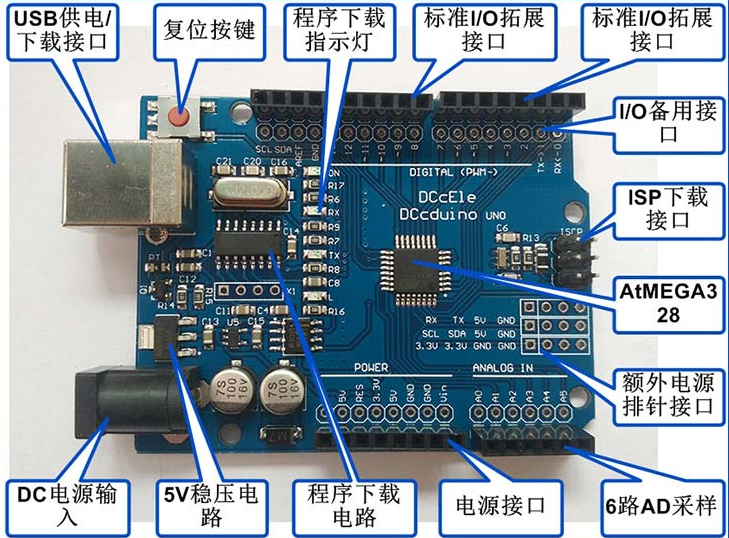
\includegraphics[width=0.85\linewidth]{figure/2-1}
	\caption{Arduino uno 单片机}
	\label{fig:2-1}
\end{figure}

\newpage
2. Arduino扩展模块---Ethernet模块

Ether扩展板如图\ref{fig:2-2}主要通过网线负责网络通信和数据传输。W5100模块是一款多功能的单片网络接口芯片,内部集成有10/100以太网控制器,主要应用于高集成、高稳定、高性能和低成本的嵌入式系统中。在本次设计中通过Ethernet模块,可将传感器数据发送至服务器,完成远程数据信息监控。

\begin{figure}[htbp]
	\centering
	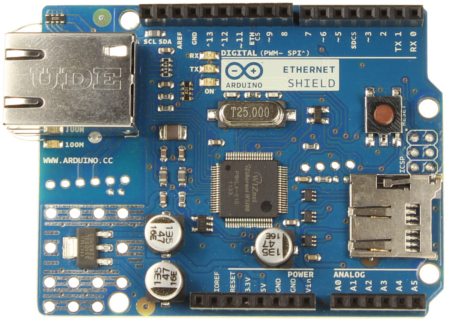
\includegraphics[width=0.85\linewidth]{figure/2-2}
	\caption{Arduino Ethernet 模块}
	\label{fig:2-2}
\end{figure}

3. Arduino传感器模块---DHT11模块,烟雾MQ2模块、红外接收发射模块。

Arduino传感器模块如图\ref{fig:2-3}负责监控和控制各个节点的环境信息。

DHT11传感器是一种温湿度复合传感器,包含标定的数字信号输出。采用专用数字化模块化采集技术和温湿度传感器技术,保证了产品极高的可靠性和长期卓越的稳定性。该传感器由电阻式感湿元件和 NTC温度测量元件组成,并与高性能8位单片机相连。这种传感器具有质量优良、响应速度快、抗干扰性强、性价比极高等优点。

MQ-2传感器是基于QM-NG1探针的气体传感器,QM-NG1是一种广谱气体传感器,采用目前国际上工艺最成熟、生产规模最大的\ce{SnO2}材料作为敏感基质制成。本产品的最大特点是对各种易燃气体(如氢、液化气、一氧化碳、烷烃等)和有毒气体(如酒精、乙醚、汽油、烟雾等)高度敏感。

红外与LED模块化是一种与Arduino兼容的红外发射传感器,通过编程发射出38 KHz的调制信号,使其能够适应市场上各种红外接收头,使红外接收器模块化的38 KHz红外接收传感器能够接收,从而实现红外无线通信。红外线发射器的核心器件是红外线发射器,广泛应用于红外遥控装置。本模块具有3 PIN接口,通过 Arduino等控制板可以方便地实现红外遥控、通信功能。红外线发射器是一种二极管,可以发射特定波长的红外光。红外线遥控器利用红外线发射器发出一连串二进制脉冲码信号。在无线传输过程中,为了避免其它红外信号的干扰,它通常是在特定载波频率上进行调制,然后通过红外二极管发射头发射出去。

\begin{figure}[htbp]
	\centering
	\subfigure[DHT11 温湿度传感器模块]{
	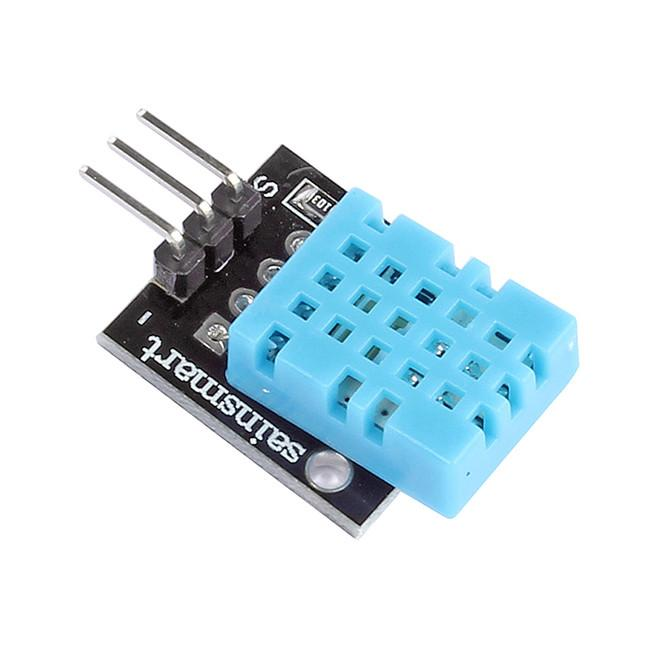
\includegraphics[width=0.3\linewidth]{figure/2-3-1}}
	\subfigure[MQ2 烟雾传感器模块]{
	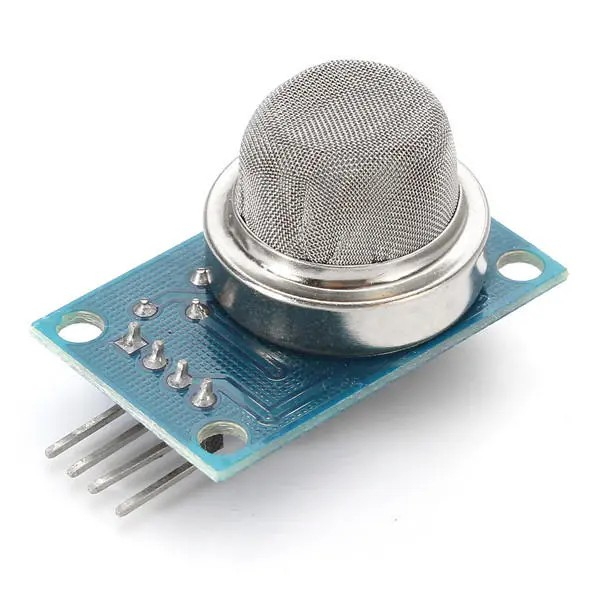
\includegraphics[width=0.3\linewidth]{figure/2-3-2}}
	\subfigure[红外接收发送模块]{
	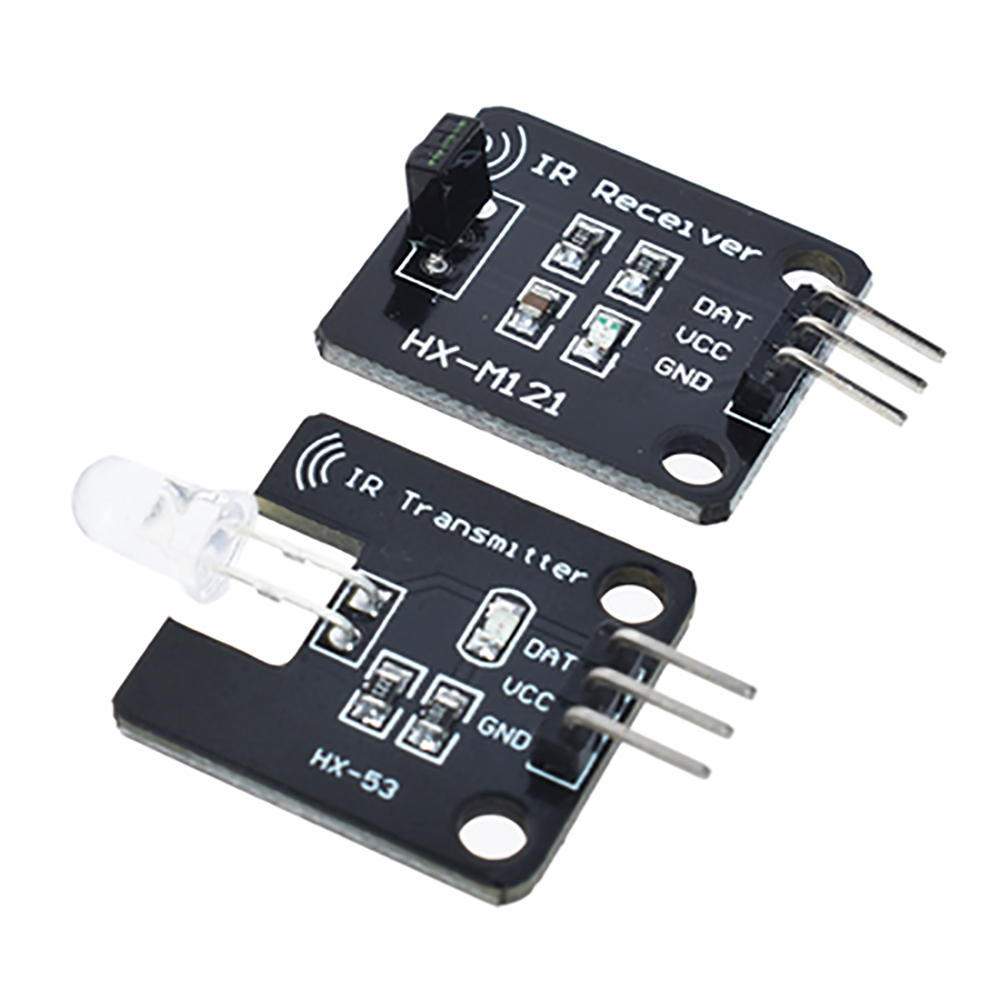
\includegraphics[width=0.3\linewidth]{figure/2-3-3}}
	\caption{传感器模块图}
	\label{fig:2-3}
\end{figure}



\subsubsection{系统架构流程设计}

本系统采用了模块化设计。对实际功能进行模块划分,明确了各模块的功能特征,为以后的开发提供了良好的功能划分。保证输出的一致性,提高设计效率,适用性强,易于维护,易于协作。按照模块化思想,确立系统的整体架构图如下图\ref{fig:2-4}所示

% 图有问题,需要修改  架构图是按功能模块划分的
\begin{figure}[htbp]
	\centering
	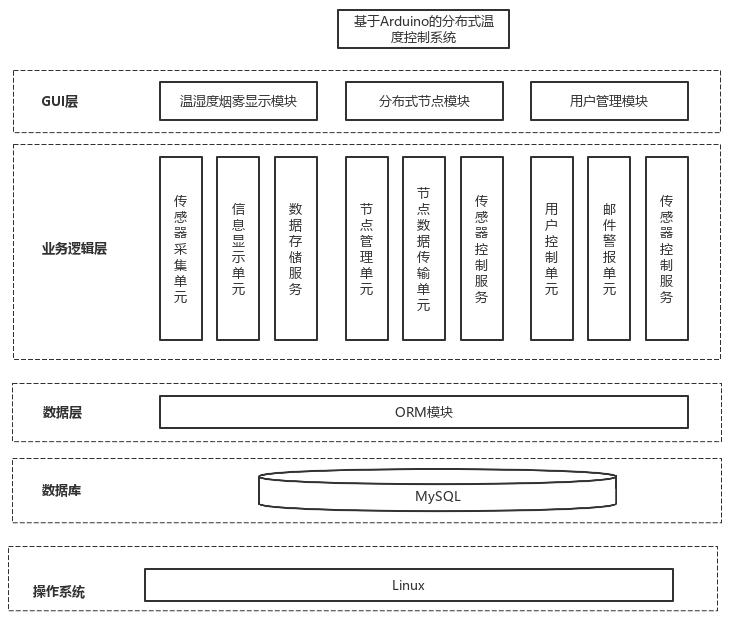
\includegraphics[width=1\linewidth]{figure/2-4}
	\caption{整体架构图}
	\label{fig:2-4}
\end{figure}

用于表达系统的逻辑信息流
用于寻找系统需求
简单、以理解的图形符号
建立手动和自动系统需求

数据流图是描述输入数据数据流到输出数据流的变换加工,进而对系统进行整体的功能建模。数据流图用来用于表达系统的逻辑信息流和寻找系统需求,通过简单、以理解的图形符号表达了系统中的据传从输入到存储间所涉及的过程。数据流中通过对数据流、加工、文件、源或宿这些数据元素的表示,反映系统必须完成的逻辑功能,确定功能模型。图\ref{fig:2-5}图\ref{fig:2-6}所示的客户端服务端交互图是需求分析阶段的成果。

从图中可以看出客户端系统主要由Arduino开发板为中心,通过Arduino开发板附加的各类扩展,完成相应的功能模块。各模块承担信息的收集、发送作用。之后Arduino开发板对数据处理后在以MQTT协议按照与服务端约定的数据格式进行发送。

服务端由MQTT服务器负责接收数据,Flask-MQTT负责数据读取,此时,为了确保数据的及时性,对传入数据立即进行判断,看是否超过设定值,选择是否触发相应警报。之后对对数据附加标注之后存入数据库。之后在由相关的模块从数据库取得各类数据,在前端页面进行可视化展示。

\begin{figure}[htbp]
	\centering
	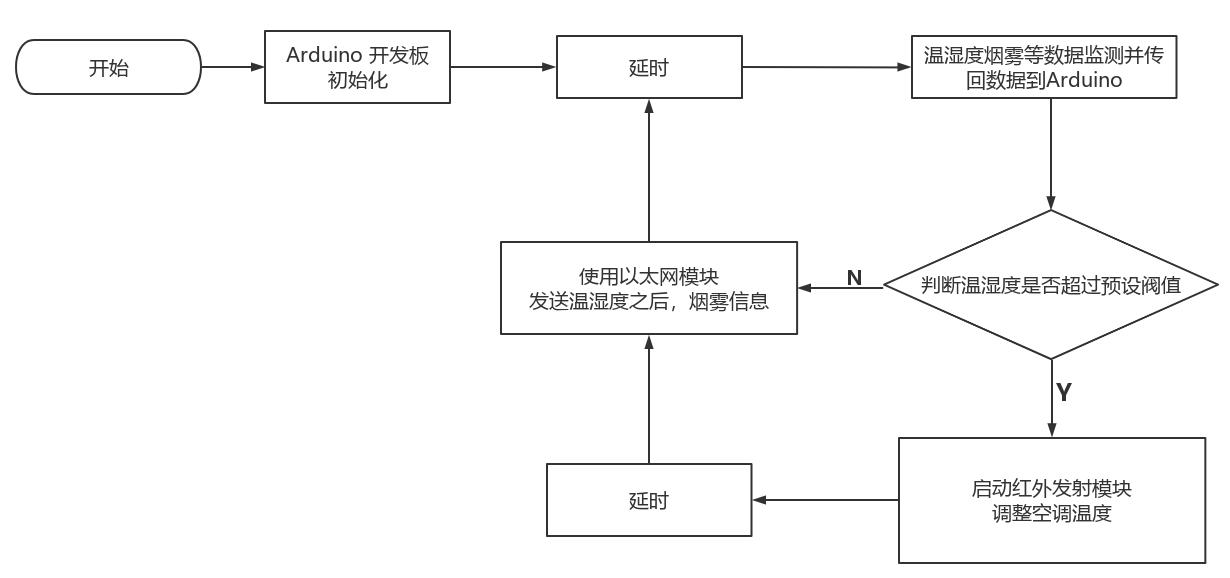
\includegraphics[width=0.85\linewidth]{figure/2-5}
	\caption{Arduino端程序流程图}
	\label{fig:2-5}
\end{figure}

\begin{figure}[htbp]
	\centering
	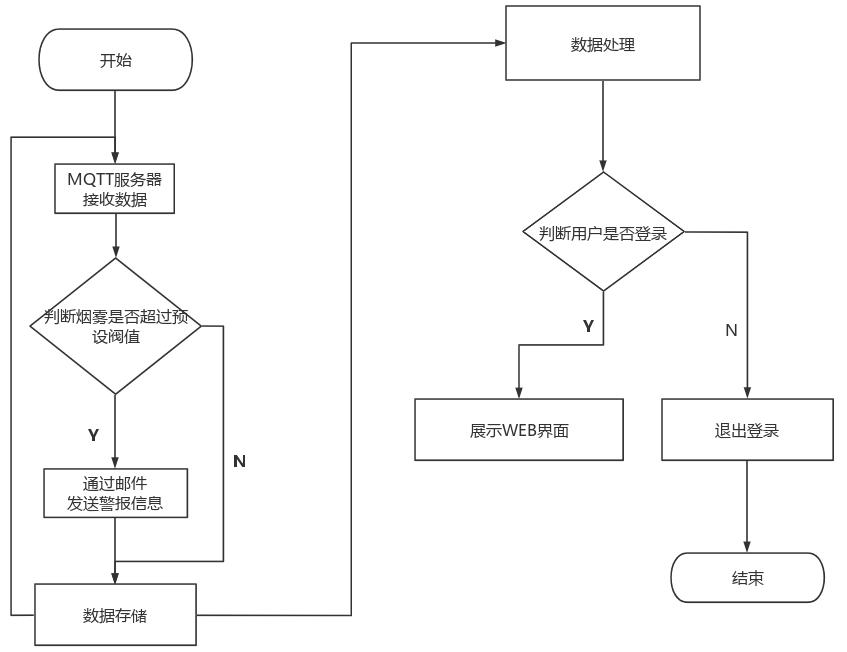
\includegraphics[width=0.85\linewidth]{figure/2-6}
	\caption{服务端流程图}
	\label{fig:2-6}
\end{figure}



\subsection{数据库设计}

数据库设计是根据数据库模型组织数据的过程。设计者确定必须存储什么数据以及数据元素是如何相互关联的。有了这些信息,我们就可以开始将数据拟合到数据库模型中。数据库设计涉及分类数据和确定相互关系。这种关于数据的理论表示被称为本体论。本体论是数据库设计背后的理论。

在大多数情况下,设计数据库的人是在数据库设计领域具有专业知识的人,而不需要业务领域的专业知识,例如,教育经验,从医经验等。因此,数据库设计必须与在该领域具有专业知识的人员合作确定,以确定必须在系统内存储什么样的数据。这是因为具有必要领域知识的人员经常无法清楚地表达他们对数据库的系统要求是什么,因为他们不习惯于根据必须存储的离散数据元素进行思考。要存储的数据可以由需求规格确定。这个过程通常被认为是需求分析的一部分。

\begin{figure}[htbp]
	\centering
	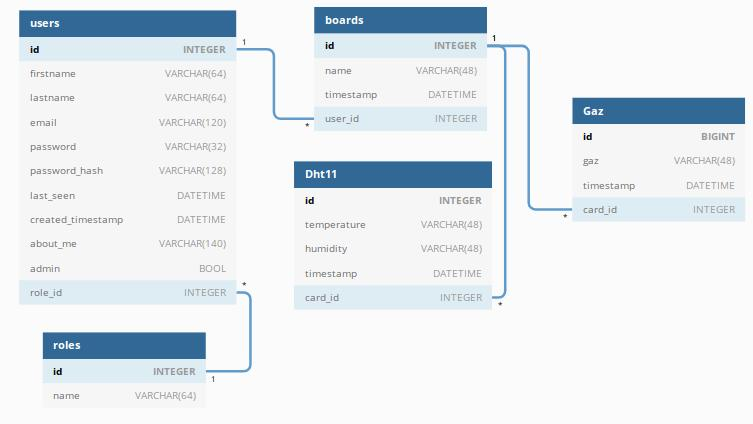
\includegraphics[width=1\linewidth]{figure/2-7}
	\caption{数据库关系图}
	\label{fig:2-7}
\end{figure}

一旦数据库设计者确定要存储在数据库中的数据后,他们就必须确定数据间的依赖关系。例如,在姓名和地址列表中,假设多人可以拥有相同的地址,但一个人不能拥有多个地址的情况下,地址取决于姓名。当提供姓名时,地址可以唯一确定,然而,反过来并不成立 —— 当给定一个地址时,名称不能唯一确定,因为多个人可以居住在一个地址。由于地址是由名称决定的,所以地址被视为取决于名称。

大多数数据库设计文件采用 
E-R图\footnote{实体 - 关系模型(简称ER模型)描述了特定知识领域中相关的感兴趣事物。基本的ER模型由实体类型(对感兴趣的事物进行分类)组成,并指定可能存在于这些实体类型的实例之间的关系。}或更直观的矢量图片表示。

本次设计的数据库关系模型如下图\ref{fig:2-7}所示。本次的数据库设计中,采用了ORM面向对象编程和关系型数据库方式进行编程操作数据库,面向对象编程把所有实体看成对象(object),关系型数据库则是采用实体之间的关系(relation)连接数据。很早就有人提出,关系也可以用对象表达,这样的话,就能使用面向对象编程,来操作关系型数据库。简单说,ORM 就是通过实例对象的语法,完成关系型数据库的操作的技术,是"对象-关系映射"(Object/Relational Mapping)的缩写。其中映射关系为:
\\ 1. 数据库的表(table)对应编程语言中的类(class)
\\ 2. 数据库中的记录(record,行数据)对应编程语言中的对象(object) 
\\ 3. 数据库中的字段(field)对应编程语言中的对象的属性(attribute)

下面以上图\ref{fig:2-7}中以User表的建立来举例:通过ORM的使用,与传统数据库操作比较就可以发现,ORM 使用对象,封装了数据库操作,因此可以不碰 SQL 语言。开发者只使用面向对象编程,与数据对象直接交互,不用关心底层数据库。

项目代码通常会使用诸如Git\footnote{Git 是一个版本控制系统,用于跟踪计算机文件中的变化并协调多人之间的这些文件的工作。在后文还会详细介绍本项目基于 Git 的团队协作工作流。}、SVN\footnote{SVN使用起来有点像是档案仓库的感觉,支持并行读写文件,支持代码的版本化管理,功能包括取出、导入、更新、分支、改名、还原、合并等。}等版本控制工具管理起来,其好处众所周知,一个是代码多版本管理,另一个是多人协作开发。在项目的持续进展中,数据库的模式(Schema)通常也经常需要更新,比如增加一个表、增加一个列或者创建一个索引等。当新版本升级发布时,在部署阶段,我们需要一个工具能够记录数据库变更版本,类似Git一样能够随时checkout到指定的数据库版本,支持upgrade以及downgrade。我们连接数据库的driver通常称为引擎(engine),这些引擎是抽象接口,其驱动的具体实现可以是mysql、sqlite等关系数据库,实际部署时通过配置的connection协议区分。因此我们的工具应该不依赖于某个具体数据库,而应该是一个通用的工具,屏蔽底层数据库的差别。而支持SQLAlchemy数据库model变更的工具我们称为数据库版本管理工具,或者称为Migrate工具。所有涉及的数据库模式变更脚本都放到称为migrate repository目录中。目前主流的两大主流Migrate工具分别为SQLAlchemy Migrate和Alembic。本次通过使用Alembic引入了可控制数据库版本的特性。

\begin{lstlisting}
op.create_table('users',
sa.Column('id', sa.Integer(), nullable=False),
sa.Column('firstname', sa.String(length=64), nullable=True),
sa.Column('lastname', sa.String(length=64), nullable=True),
sa.Column('email', sa.String(length=120), nullable=True),
sa.Column('password', sa.String(length=32), nullable=True),
sa.Column('password_hash', sa.String(length=128), nullable=True),
sa.Column('last_seen', sa.DateTime(), nullable=True),
sa.Column('created_timestamp', sa.DateTime(), nullable=True),
sa.Column('about_me', sa.String(length=140), nullable=True),
sa.Column('admin', sa.Boolean(), nullable=True),
sa.Column('role_id', sa.Integer(), nullable=True),
sa.ForeignKeyConstraint(['role_id'], ['roles.id'], ),
sa.PrimaryKeyConstraint('id')
)
\end{lstlisting}


	%\pagenumbering{arabic}
\section{开发技术选择}

\subsection{物联网通讯协议  MQTT}

在本系统前期的网络数据传输技术选型对比了TCP/UDP/JSON/MQTT等传输协议或方式的优缺点,综合考虑选择了MQTT(Message Queuing Telemetry Transport,消息队列遥测传输协议)作为本次客户端节点和服务端节点数据交互的协议。其协议广泛应用于机器对机器(M2M)/物联网(IoT)的应用层连接协议,使用极其轻量级的发布/订阅二进制消息模型通信。对于需要较小代码占用空间和或网络带宽非常宝贵的远程连接非常有用,是专为受限设备(电池功率非常高的移动应用设备)和低带宽、高延迟或不可靠的环境通信而设计的。不仅为新兴的“机器到机器”(M2M)或物联网(IoT)世界提供连接,还被用于通过卫星链路与代理通信的传感器、与医疗服务提供者的拨号连接以及一系列家庭自动化和小型设备场景。
\\ 相对与其他协议,MQTT具有以下特性:
\\1. 底层基于TCP/IP (或者UDP) 协议传输,采用发布/订阅模式的二进制消息模式,提供一对多的消息发布
\\2. 控制包结构精简,第一个 1字节固定报头,第二个2字节心跳报文,最小化传输开销和协议交换,有效减少网络流量。
\\3. 消息QoS支持,可靠性传输保证(TCP协议传输)
\\4. 使用Last Will和Testament特性通知有关各方客户端异常中断的机制。

MQTT 协议主要有三大核心角色:发布者(Publisher)、Broker代理服务器(转发者)、订阅者(Subscriber)。其中消息的发布者和订阅者都是客户端角色,消息代理是服务器,消息发布者可以同时是订阅者。

MQTT客户端身兼二职:既可以是发布者角色,又可以是订阅者角色。一个使用MQTT协议的应用程序或者设备就是一个MQTT 客户端,工作时它需要主动去连接到代理服务器。

MQTT服务器又称为"消息代理"服务器(Broker),可以是一个应用程序或一台设备,它是位于消息发布者和订阅者之间,具有以下功能:
接受来自客户端的网络连接并建立通信链路,
接收发布者的主题(Topic)并转发给订阅者,
处理来自客户端的订阅和退订请求,
向订阅的客户转发相应地主题(Topic)。其具体交互流程如下图\ref{fig:3-1}所示:

\begin{figure}[htbp]
	\centering
	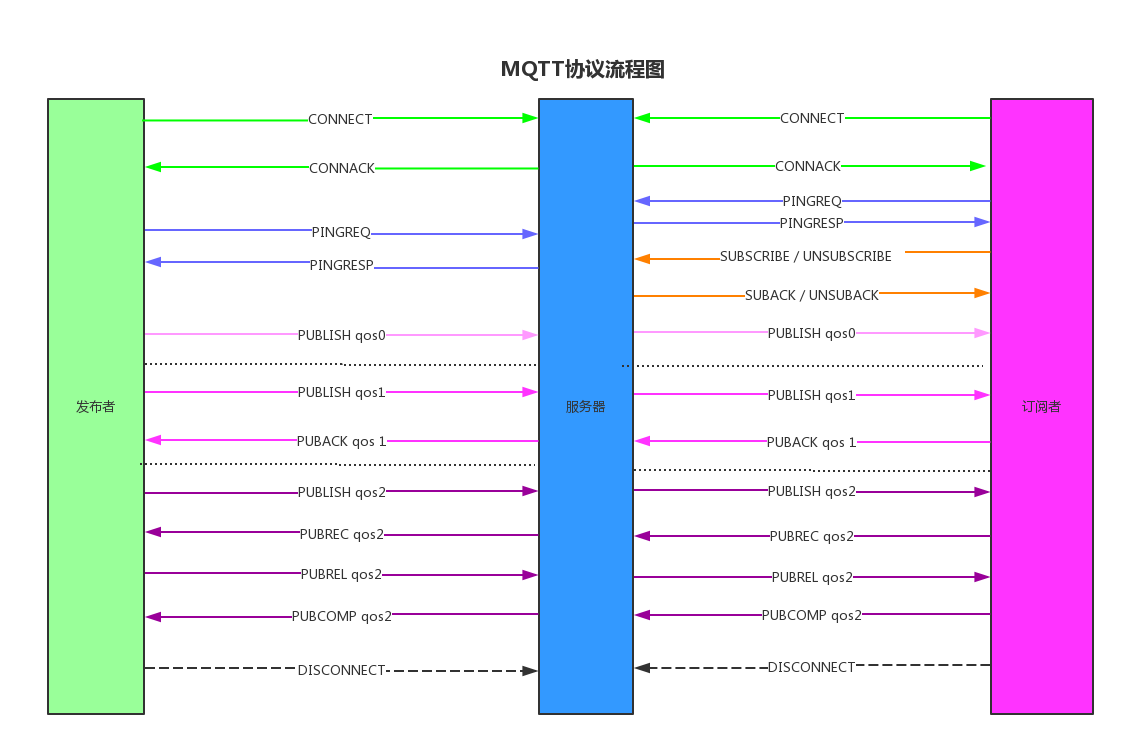
\includegraphics[width=1\linewidth]{figure/3-1}
	\caption{MQTT协议流程图}
	\label{fig:3-1}
\end{figure}


\subsection{关系性数据库 MySQL}


数据库(Database)是按照数据结构来组织、存储和管理数据的仓库。
每个数据库都有一个或多个不同的 API 用于创建,访问,管理,搜索和复制所保存的数据。
我们也可以将数据存储在文件中,但是在文件中读写数据速度相对较慢。
所以,现在我们使用关系型数据库管理系统(RDBMS)来存储和管理大数据量。所谓的关系型数据库,是建立在关系模型基础上的数据库,借助于集合代数等数学概念和方法来处理数据库中的数据。
\\RDBMS 即关系数据库管理系统(Relational Database Management System)的特点:

1.数据以表格的形式出现

2.每行为各种记录名称

3.每列为记录名称所对应的数据域

4.许多的行和列组成一张表单

5.若干的表单组成database


MySQL 是一个关系型数据库管理系统,由瑞典 MySQL AB 公司开发,目前属于 Oracle 公司。MySQL 是一种关联数据库管理系统,关联数据库将数据保存在不同的表中,而不是将所有数据放在一个大仓库内,这样就增加了速度并提高了灵活性。
MySQL具有以下特性:
\begin{itemize}
	\item MySQL 是开源的,目前隶属于 Oracle 旗下产品。
	\item MySQL 支持大型的数据库。可以处理拥有上千万条记录的大型数据库。
	\item MySQL 使用标准的 SQL 数据语言形式。
	\item MySQL 可以运行于多个系统上,并且支持多种语言。这些编程语言包括 C、C++、Python、Java、Perl、PHP、Eiffel、Ruby 和 Tcl 等。
	\item MySQL 支持大型数据库,支持 5000 万条记录的数据仓库,32 位系统表文件最大可支持 4GB,64 位系统支持最大的表文件为8TB。
	\item MySQL 是可以定制的,采用了 GPL 协议,可以修改源码来开发自己的 MySQL 系统。
\end{itemize}

\subsection{Python开发语言 Flask模块}

Flask一直被称为是Python中轻量级的可定制的框架,其核心简单,相比其他框架更加灵活轻便,也更容易掌握。

你能Flask框架核心简单,同时在使用过程同样可以保持功能的丰富与扩展性,用户在使用Flask开发网站时,可以根据自己的需求添加不同的功能,各种强大的插件库可以让用户完全按照自己的意愿开发出功能强大的为国内站。

\begin{lstlisting}[title=代码 3-1:Flask简单示例]
from flask import Flask
app = Flask(__name__)
@app.route('/')
def index():
    return 'Hello World'
\end{lstlisting}

仅仅5行代码,就可以在浏览器中显示一个Hello World响应。所以Flask的其中一个优势再明显不过了:简洁。且不说Java的Web框架Spring,就说同样使用Python的框架Django,写一个Hello World程序也得10行代码。

第一行,导入包。

第二行,创建对象。

第三行,创建路由。

第四行、第五行,视图函数。

\subsection{SQLAlchemy---对象关系映射器(ORM)}

SQLAlchemy是一个功能非常强大的库,用于在Python中处理关系数据库。代替手工编写SQL查询,我们可以使用普通的Python对象来表示数据库表并执行查询。这种方法有很多好处,如下代码所示:

\begin{lstlisting}[title=DHT11数据表对象数据表模型]
class Dht11(PaginatedAPIMxin, db.Model):
__tablename__ = 'Dht11'
id = db.Column(db.Integer, primary_key=True)  #卡片存储收到MQTT数据的序号
temperature = db.Column(db.String(48), index=True) #存储MQTT数据中温度
humidity = db.Column(db.String(48), index=True)  #存储MQTT数据中湿度
timestamp = db.Column(db.DateTime, index=True, default=datetime.utcnow) #存储当前收到数据的时间戳
card_id = db.Column(db.Integer, db.ForeignKey('boards.id')) #对应的卡片ID

def __repr__(self):   #__repr__方法,它用于生成Dht11类实例的辅助显示内容
	return '<temp:{0}, humidity:{1}'.format(self.temperature, self.humidity)

def to_dict(self):  #单个对象方法
	data = {
		'id_from_db': self.id,
		'owner_email': str(User.query.get_or_404(self.card_id).email),
		'from_card_id': self.card_id,
		'value_created_at': self.timestamp,
		'temperature': self.temperature,
		'humidity': self.humidity,
		'_links': {
			(self.card_id).id) # user_id
			}
		}
	return data
\end{lstlisting}

通过ORM方法的使用很容易的构建了返回对象的数据格式

与手工编写SQL查询相反,我们可以使用普通的Python对象来表示数据库表,并执行查询。如下,该方法有很多的优点:

应用程序可以完全用Python开发。

数据库引擎之间的细微差别被抽象掉了。这使可以像处理轻量级数据库一样进行操作,例如,使用SQLite进行本地开发和测试,然后切换到专为生产中的高负载而设计的数据库(例如PostgreSQL)。

数据库错误不太常见,因为您的应用程序和数据库服务器之间现在存在两层:Python解释器本身(这将捕获明显的语法错误)和SQLAlchemy,后者具有定义良好的API和自己的错误检查层。

由于SQLAlchemy的工作单元模型有助于减少不必要的数据库往返次数,因此数据库代码可能会变得更加高效。SQLAlchemy还具有有效地预取相关对象的功能,称为预先加载。

对象关系映射(Object Relational Mapping,ORM)使代码更具可维护性,这被称为“不要重复自己”(DRY)。假设将列添加到模型中。使用SQLAlchemy,只要您使用该模型,它将可用。另一方面,如果整个应用程序中都散布着手写的SQL查询,则需要一次更新一次每个查询,以确保包含新列。SQLAlchemy可以帮助避免SQL注入漏洞。

出色的库支持:有很多有用的库可以直接与SQLAlchemy模型一起使用,以提供诸如维护接口和RESTful API之类的东西。

应用可以完全使用Python开发。


\subsection{RESTful 架构开发方式}
REST全称是Representational State Transfer,中文意思是表述(通常译为表现层状态转移)。 REST本身并没有创造新的技术、组件或服务,而隐藏在RESTful背后的理念就是使用Web的现有特征和能力, 更好地使用现有Web标准中的一些准则和约束。虽然REST本身受Web技术的影响很深, 但是理论上REST架构风格并不是绑定在HTTP上,只不过目前HTTP是唯一与REST相关的实例。 所以我这里描述的REST也是通过HTTP实现的REST。

REST全称是表述性状态转移,那究竟指的是什么的表述? 其实指的就是资源。任何事物,只要有被引用到的必要,它就是一个资源。资源可以是实体(例如手机号码),也可以只是一个抽象概念(例如价值) 。下面是一些资源的例子:
\begin{itemize}
	\item 某用户的手机号码
	\item 某用户的个人信息
\end{itemize}

要让一个资源可以被识别,需要有个唯一标识,在Web中这个唯一标识就是URI(Uniform Resource Identifier)。

URI既可以看成是资源的地址,也可以看成是资源的名称。如果某些信息没有使用URI来表示,那它就不能算是一个资源, 只能算是资源的一些信息而已。URI的设计应该遵循可寻址性原则,具有自描述性,需要在形式上给人以直觉上的关联。这里以github网站为例,给出一些还算不错的URI:
\begin{itemize}
	\item https://github.com/git/git
	\item https://github.com/git/git/blob/master/block-sha1/sha1.h
	\item https://github.com/git/git/commit/e3af72cdafab5993d18fae056f87e1d675913d08
	\item https://github.com/git/git/pulls
	\item https://github.com/git/git/pulls?state=closed
\end{itemize}

1. REST描述的是在网络中client和server的一种交互形式;REST本身不实用,实用的是如何设计 RESTful API(REST风格的网络接口);
2. Server提供的RESTful API中,URL中只使用名词来指定资源,原则上不使用动词。“资源”是REST架构或者说整个网络处理的核心。
比如:
\begin{itemize}
	\item http://api.qc.com/v1/newsfeed: 获取新闻; 
	\item http://api.qc.com/v1/friends: 获取某人的好友列表;
	\item http://api.qc.com/v1/profile: 获取某人的详细信息;
\end{itemize}

3. 用HTTP协议里的动词来实现资源的添加,修改,删除等操作。即通过HTTP动词来实现资源的状态扭转:GET 用来获取资源,POST 用来新建资源(也可以用于更新资源),PUT 用来更新资源,DELETE 用来删除资源。比如:
\begin{itemize}
	\item DELETE http://api.qc.com/v1/friends: 删除某人的好友 (在http parameter指定好友id)
	\item GET  http://api.qc.com/v1/friends: 请求好友资料
	\item POST http://api.qc.com/v1/friends: 添加好友
	\item UPDATE http://api.qc.com/v1/profile: 更新个人资料
\end{itemize}

如下图\ref{fig:3-2}例:
\begin{figure}[H]
	\centering
	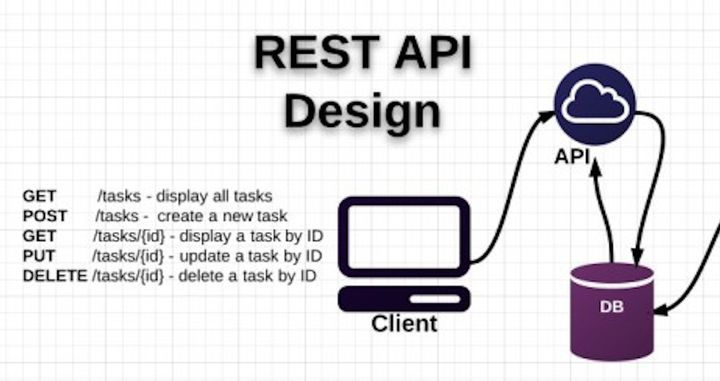
\includegraphics[width=0.85\linewidth]{figure/3-2}
	\caption{RESTful 设计理念图}
	\label{fig:3-2}
\end{figure}

通过使用RESTful可以做到:前后端分离,减少流量。
安全问题集中在接口上,由于接受json格式,防止了注入型等安全问题。
前端无关化,后端只负责数据处理,前端表现方式可以是任何前端语言(android,ios,html5)。
前端和后端人员更加专注于各自开发,只需接口文档便可完成前后端交互,无需过多相互了解。
服务器性能优化:由于前端是静态页面,通过nginx便可获取,服务器主要压力放在了接口上。

	\section{系统开发与实现}

\subsection{结构化开发方式}

结构化方法是一种传统的软件开发方法,它是由结构化分析、结构化设计和结构化程序设计三部分有机组合而成的。结构化设计方法是以自顶向下,逐步求精,模块化为基点,以模块化,抽象,逐层分解求精,信息隐蔽化局部化和保持模块独立为准则的设计软件的数据架构和模块架构的方法学。它的要点是是把一个复杂问题的求解过程分阶段进行,而且这种分解是自顶向下,逐层分解,使得每个阶段处理的问题都控制在容易理解和处理的范围内。

结构化方法的基本思想主要体现在三个方面。

(1)自顶向下,逐步求精:把程序看成是一个逐步演化的过程。把一个系统与程序看成是一层一层的。本次的系统开发中,按照自顶向下方式。基于Arduino的分布式温度控制系统可分为:数据收集,数据传输,数据展示,用户管理等几个子系统,而每个子系统又划分为接收/发送信息,实施处理,提供返回信息等等部分。

(2)模块化:即将几个系统分成几个模块,每个模块实现特定的功能,最终整个系统由这些模块组成。模块跟模块之间通过接口传递信息,模块最重要的特点就是独立性,模块之间还有上下层的关系,上层模块调用下层模块来实现一些功能。本系统的模块化图如下图\ref{fig:4-1}所示

\begin{figure}[htbp]
	\centering
	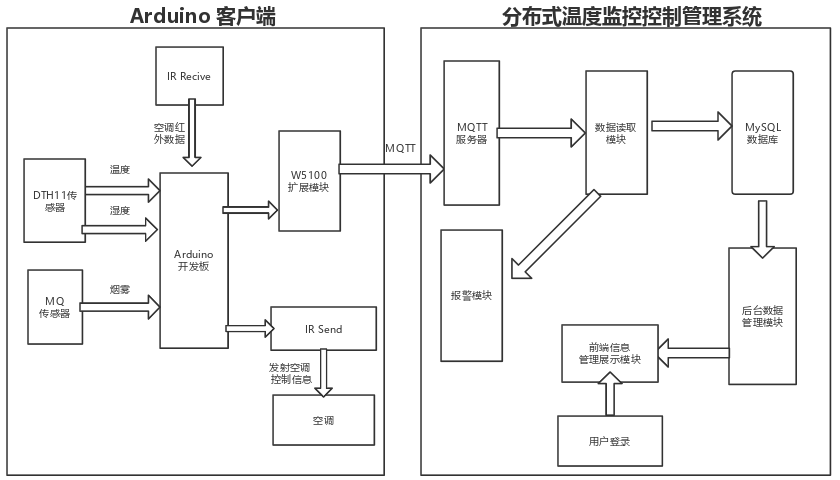
\includegraphics[width=\linewidth]{figure/4-1}
	\caption{温度控制系统模块图}
	\label{fig:4-1}
\end{figure}

(3)语句结构化:顺序结构、分支结构、循环结构,都是常用的语句结构。

结构化分析方法的实质是着眼于数据流,自顶向下,逐层分解,建立系统的处理流程,以数据流图和数据字典为主要工具,建立系统的逻辑模型。

结构化分析的步骤如下:

(1)通过对计划任务书的需求分析为背景,确立整个系统的具体模型

(2)去掉具体模型中非本质因素,抽象出当前系统的逻辑模型

(3)根据计算机的特点分析当前系统与目标系统的差别,建立目标系统的逻辑模型

(4)完善目标系统并补充细节,写出目标系统的软件需求规格说明

(5)测试直到确认满足计划任务书对软件的需求

结构化设计方法给出一组帮助设计人员在模块层次上区分设计质量的原理与技术。它通常与结构化分析方法衔接起来使用,以数据流图为基础得到软件的模块结构。SD方法尤其适用于变换型结构和事务型结构的目标系统。在设计过程中,它从整个程序的结构出发,利用模块结构图表述程序模块之间的关系。


% \subsection{基于 Git 的版本控制和多人协作}

% Git 是一个版本控制系统,用于跟踪计算机文件的变化,并在多个人员之间协调对这些文件的工作。它主要用于软件开发中的源代码版本控制,同时它也可以用来跟踪我们的任何一个文件的变化过程。作为一个分布式的版本控制系统,它的主要特性是高速、数据完整性和对分布式、非线性工作流的支持。

% Git 是由 Linus Torvalds 在 2005 年创建的,当时用于开发 Linux 内核,其他内核开发人员也为其最初的开发做出了贡献。Junio Hamano则是目前的维护者。Git 不同与大多数客户机 — 服务器系统(C/S System),每个计算机上的每个 Git 目录都是一个完整的存储库,具有完整的历史和完整的版本跟踪功能,独立于网络访问或中央服务器。

% 如图 \ref{git-flow} 所示,Git 的最大优点之一是它的分支功能。与其他集中式的版本控制系统的不同点在于,Git 分支是廉价且易于合并的。这使得特性分支工作流受到许多 Git 用户的欢迎。
% 特性分支为代码库的每个更改提供一个隔离的环境。当一个开发人员想要开始做一些事情 —— 不管他们有多大或多么小的时候 —— 他们会创建一个新的分支。这确保了主分支总是包含生产质量代码。

% \begin{figure}
% 	\centering
% 	\includegraphics[width=0.6\linewidth]{figure/git-flow}
% 	\caption{基于 Git 的工作流}
% 	\label{git-flow}
% \end{figure}

% 使用特性分支不仅比直接编辑生产代码更可靠,而且还提供了有组织的开发。例如,在之后针对本系统的完善时可以新建feature分支,代成熟后在和入主分支。确保了主分支的稳健性。

% 特性分支、分布式开发、Pull Request 和稳定的社区环境的最终结果是一个更快的发布周期。这些功能促进了敏捷的工作流,鼓励开发人员更频繁地共享较小的更改。例如,我们可以配置 Git,以便在任何人将一个 pull 请求合并到测试服务器时,将最新的提交从开发分支部署到测试服务器。将这种构建自动化与单元测试结合,让代码从开发阶段转向生产阶段时,对代码质量拥有最高的信心。

% Git 在用户如何管理更新方面提供了很大的灵活性。当在 Git 中与团队合作开发时,确保团队的开发方向是非常重要的。本系统的代码已在在线代码托管平台提供商码云(Gitee)\footnote{基于Arduino的分布式温度控制系统开源地址:\url{https://gitee.com/xsyu_security/arduino.io}}全部开源。
% 选择码云服务主要原因在于:

% \begin{itemize}
% 	\item 国内的Git服务拥有更快的访问速度
% 	\item 私有库功能对个人开发者免费
% 	\item 线上自动代码质量分析
% 	\item 中文语言便于团队成员上手
% \end{itemize}

% Git非常受欢迎,被广泛使用,并被开发人员社区中绝大多数人接受为标准版本控制系统。在大量的Git用户组成的社区可以让我们寻求外部帮助并轻松解决问题。答辩系统业务的开发严重依赖于软件开发流程,Git将彻底改变了我们团队创建和交付工作的方式。包括设计、开发、产品管理、上线运行、客户支持在内的各种流程都可以在开发团队中使用Git轻松处理和维护。

\subsection{红外编码}
红外通信是利用近红外波段的红外线作为传递信息的媒体,即通信信道。发送端将基带二进制信号调制为一系列的脉冲串信号,通过红外发射管发射红外信号。接收端将接收到的光脉转换成电信号,再经过放大、滤波等处理后送给解调电路进行解调,还原为二进制数字信号后输出。常用的有通过脉冲宽度来实现信号调制的脉宽调制(PWM)和通过脉冲串之间的时间间隔来实现信号调制的脉时调制(PPM)两种方法。 简而言之,红外通信的实质就是对二进制数字信号进行调制与解调,以便利用红外信道进行传输;红外通信接口就是针对红外信道的调制解调器。二进制数字信号如何进行调制与解调,利用何种红外信道进行传输,这就被称为红外协议。因为在后续空调解码器的设计中需要甄别不同的协议,所以下文将详细介绍几种常见的红外通信协议:

1. NEC 协议的基本特征:
	8 位地址位,8 位命令位。
	为了可靠性地址位和命令位被传输两次。
	脉冲位置调制。
	载波频率38kHz。
	每一位的时间为1.125ms 或 2.25ms。

逻辑 0 和 1 的定义:
\begin{itemize}
	\item 逻辑 1 的是由560$\mu$s的高电平和1.69ms的低电平组成的脉冲表示。
	\item 逻辑 0 的是由560$\mu$s的高电平和565$\mu$s的低电平组成的脉冲表示。
\end{itemize}
\begin{figure}[htbp]
	\centering
	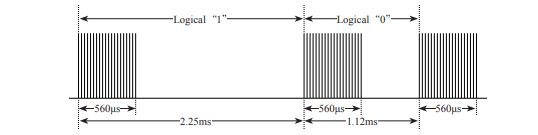
\includegraphics[width=\linewidth]{figure/4-2}
	\caption{NEC的0,1码}
	\label{fig:4-2}
\end{figure}

重复码的格式是由9ms的高电平和2.25ms 的低电平及一个560$\mu$s的高电平组成

发送格式如下:
NEC 协议中,首先是9ms的高电平脉冲,其后是 4.5ms 的低电平,接下来就是 8bit 的地址码(从低有效位开始发),而后是 8bit 的地址码的反码(主要是用于校验是否出错)。然后是 8bit 的命令码(也是从低有效位开始发),而后也是 8bit 的命令码的反码。
\begin{figure}[htbp]
	\centering
	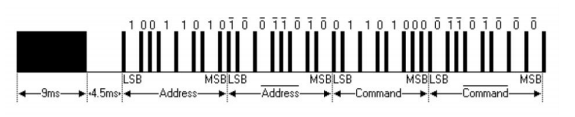
\includegraphics[width=\linewidth]{figure/4-3}
	\caption{NEC编码}
	\label{fig:4-3}
\end{figure}

2. RC5 协议
RC5 协议由 Philips 公司推出。它采用载波频率固定为36kHz 的 ASK 调制和曼彻斯特编码。
基本特征:
(1)4 位地址位,4 位命令位。
(2)地址位和命令位被传输一次。
(3)载波频率36kHz。
(4)每一位的时间为1.05ms 或 2.1ms。

逻辑 0 和 1 的定义如:
逻辑 1 的是由889$\mu$s 的低电平和889$\mu$s 的高电平组成的脉冲表示。
逻辑 0 的是由889$\mu$s 的高电平和889$\mu$s 的低电平组成的脉冲表示。
\begin{figure}[htbp]
	\centering
	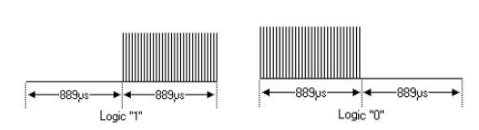
\includegraphics[width=\linewidth]{figure/4-4}
	\caption{RC5的0,1编码}
	\label{fig:4-4}
\end{figure}

发送格式如下:
RC5 协议中,首先是“110”的信号,接下来就是 5bit 的地址码。然后是 7bit 的命令码。
\begin{figure}[htbp]
	\centering
	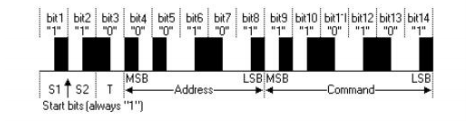
\includegraphics[width=\linewidth]{figure/4-5}
	\caption{RC5编码}
	\label{fig:4-5}
\end{figure}

为了提高红外编码的识别效率,需要引用一个IRremote库函数。在编写基于红线传感器收发通信的Arduino应用程序时,这个开源库函数可极大地减少我们的编码工作量和程序代码量。库函数硬件上支持多种Arduino主控板,软件上支持多种红外遥控编码的发送和接收协议,而且便于扩展和用户自定义。

本次系统开发过程中,针对通用空调红外遥控器,编写了以下Arduino的红外解码程序用于控制空调温度:
\begin{lstlisting}[language=C,title=代码4-1: Arduino的红外解码程序]
#include <Arduino.h>

/*
	* Define macros for input and output pin etc.
	*/
#include "PinDefinitionsAndMore.h"

/*
	* You can change this value accordingly to the receiver module you use.
	* The required value can be derived from the timings printed here.
	* Keep in mind that the timings may change with the distance
	* between sender and receiver as well as with the ambient light intensity.
	*/
#define MARK_EXCESS_MICROS    20 // recommended for the cheap VS1838 modules

//#define RECORD_GAP_MICROS 12000 // Activate it for some LG air conditioner protocols
#include <IRremote.h>

//+=============================================================================
// Configure the Arduino
//
void setup() {
	pinMode(LED_BUILTIN, OUTPUT);

	Serial.begin(9600);   // Status message will be sent to PC at 9600 baud
#if defined(__AVR_ATmega32U4__) || defined(SERIAL_USB) || defined(SERIAL_PORT_USBVIRTUAL)  || defined(ARDUINO_attiny3217)
	delay(4000); // To be able to connect Serial monitor after reset or power up and before first print out. Do not wait for an attached Serial Monitor!
#endif
	// Just to know which program is running on my Arduino
	Serial.println(F("START " __FILE__ " from " __DATE__ "\r\nUsing library version " VERSION_IRREMOTE));

	IrReceiver.begin(IR_RECEIVE_PIN, ENABLE_LED_FEEDBACK); // Start the receiver, enable feedback LED, take LED feedback pin from the internal boards definition

	Serial.print(F("Ready to receive IR signals at pin "));
	Serial.println(IR_RECEIVE_PIN);
}

//+=============================================================================
// The repeating section of the code
//
void loop() {
	if (IrReceiver.decode()) {  // Grab an IR code
		// Check if the buffer overflowed
		if (IrReceiver.decodedIRData.flags & IRDATA_FLAGS_WAS_OVERFLOW) {
			Serial.println("IR code too long. Edit IRremoteInt.h and increase RAW_BUFFER_LENGTH");
		} else {
			Serial.println();                               // 2 blank lines between entries
			Serial.println();
			IrReceiver.printIRResultShort(&Serial);
			Serial.println();
			Serial.println(F("Raw result in internal ticks (50 us) - with leading gap"));
			IrReceiver.printIRResultRawFormatted(&Serial, false); // Output the results in RAW format
			Serial.println(F("Raw result in microseconds - with leading gap"));
			IrReceiver.printIRResultRawFormatted(&Serial, true);  // Output the results in RAW format
			Serial.println();                               // blank line between entries
			Serial.print(F("Result as internal ticks (50 us) array - compensated with MARK_EXCESS_MICROS="));
			Serial.println(MARK_EXCESS_MICROS);
			IrReceiver.compensateAndPrintIRResultAsCArray(&Serial, false); // Output the results as uint8_t source code array of ticks
			Serial.print(F("Result as microseconds array - compensated with MARK_EXCESS_MICROS="));
			Serial.println(MARK_EXCESS_MICROS);
			IrReceiver.compensateAndPrintIRResultAsCArray(&Serial, true); // Output the results as uint16_t source code array of micros
			IrReceiver.printIRResultAsCVariables(&Serial);  // Output address and data as source code variables

			IrReceiver.compensateAndPrintIRResultAsPronto(&Serial);
//        }
		}
		IrReceiver.resume();                            // Prepare for the next value
	}
}
\end{lstlisting}

\subsection{对开源项目的有效利用}

开放源代码软件(OSS)是一种计算机软件,其源代码提供许可证,版权持有者有权为任何目的研究,更改和分发软件给任何人。开源软件可能会以公开的协作方式开发。根据研究它的科学家,开源软件是开放式协作的一个突出例子。

对于开发者而言,了解并使用目前在社区中比较流行的开源项目是很必要的一件事。利用这些项目,项目开发工作有时能达到事半功倍的效果。尤其是在互联网这个飞速发展的领域,快速开发、快速上线就是生命,引入开源项目可以节省很多的人力和时间,降低开发成本。Standish Group 2008年的一份报告指出,采用开源软件模式每年可为消费者节省约600亿美元(480亿英镑)的费用。但采用开源软件的决定不应仅仅以低成本为基础。在切换到开源以充分利用它之前,需要对需求进行详细的分析和理解。

包管理器是现在 web 开发必须使用的工具,因为网站系统的开发有必要借助数以万计的众多开源爱好者们的力量。本系统由以下包管理系统提供支持:Python的包安装程序 pip,Ubuntu Linux发行版的包管理器APT。pip是Python官方推荐的包管理工具:属于python的一部分。pip 也支持直接从文件读取包列表以便批量安装,通常命名为 requirements.txt。下面列出了本系统全部所用的python模块。通过requirements.txt可以方便有效的做出系统的迁移部署。APT可以方便快捷的部署各种类型服务,如本系统中采用的MQTT服务器,WEB服务器等。都可以直接通过\begin{lstlisting}[language=bash]
apt install mosquitto nginx
\end{lstlisting}一句命令直接安装,免去了windows系统下,寻找,下载,安装的方式,节省了大量的时间。

\begin{lstlisting}[title=温控系统所选用的全部Python模块以及版本列表]
alembic==1.0.10
aniso8601==7.0.0
Click==7.0
Flask==1.0.3
Flask-Admin==1.5.3
Flask-Login==0.4.1
Flask-Migrate==2.5.2
Flask-MQTT==1.0.5
Flask-RESTful==0.3.7
Flask-Restless==0.17.0
Flask-SocketIO==4.2.0
Flask-SQLAlchemy==2.4.0
Flask-WTF==0.14.2
itsdangerous==1.1.0
Jinja2==2.10.1
Mako==1.0.12
MarkupSafe==1.1.1
mimerender==0.6.0
paho-mqtt==1.4.0
python-dateutil==2.8.0
dj-database-url==0.5.0
python-editor==1.0.4
python-engineio==3.9.0
python-mimeparse==1.6.0
python-socketio==4.3.0
pytz==2019.2
six==1.12.0
SQLAlchemy==1.3.4
typing==3.7.4
Werkzeug==0.15.4
WTForms==2.2.1
gunicorn==20.1.0 
mysqlclient==1.4.2.post1
requests==2.22.0
\end{lstlisting}

上表列出了温控系统所选用的全部Python模块以及版本列表,可以看到数目相当多,而正是利用了这些方便的开源项目,才使得快速开发一个稳定、强大的温控系统成为可能。

需要注意的是,开源许可软件大多免费提供,但这不一定是这种情况。某些仅允许非商业性质的再分发,或修改源代码仅供个人使用的软件并不属于开源。开放源代码可能有一些限制,特别是关于表达对软件起源的限制,例如要求在代码中保留作者姓名和版权声明,或者要求重新分发许可软件仅在相同的许可证下发布。

本次系统的开发遵循了开源许可协议,其诞生离不开众多开源项目的支持,在此对这些开源项目作者所做出的工作表示感谢。

	\section{系统开发成果}

对基于Arduino的分布式温度控制系统已完成基本设计与开发,通过测试并于 2021 年 5 月运行在西安石油大学校内,校内网网址:\underline{http://arduino.deconf.xyz/}。将在机房自动化,校园环境智能化方面推进智能化校园建设。

\subsection{预期目标}

整体来说,本次系统设计和开发基本达成预期目标。

1. 提供了WEB页面可视化的管理和配置功能。可配置用户信息,节点信息等。

2. 关键信息的统计展示功能。完成了节点的温度、湿度、烟雾等信息的展示功能

3. 温度控制功能方面,通过Arduino传感器采集到的温度,在设定的阈值的控制下,通过红外发射模块,控制空调的温度。

3. 告警方面,在烟雾的值超过阈值之后,可以根据用户信息的电子邮箱发送对应的的告警信息。

\subsection{分布式节点管理控制系统}

依照前面的需求分析,系统设计等工作,确立了本系统采用C/S模型,来进行对各个节点的数据管控。按照前图\ref{fig:4-1}所示,进行S端的开发成果如下:

\subsubsection{用户模块}
按照模块化设计思想,实现用户模块如下所示。WEB端具有用户登录,用户注册,用户管理等功能。
用户登录具有用户鉴权,用户密码鉴别的能力,确保正确用户登录。用户注册可以使该系统支持多用户,且每个用户拥有属于自己的个人信息,以及关联的卡片信息等。用户管理方便管理员对多用户的修改,增加,删除等。用户的信息写入在后端存储的MySQL数据库中。在前端显示上做到了简洁大方以及美观。

\begin{figure}[htbp]
	\centering
	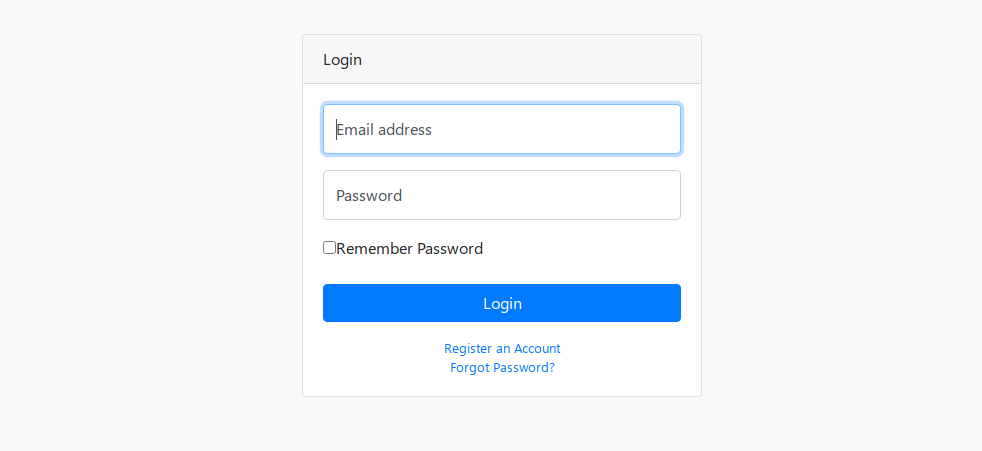
\includegraphics[width=0.85\linewidth]{figure/5-1}
	\caption{用户登录页面}
\end{figure}
\begin{figure}[H]
	\centering
	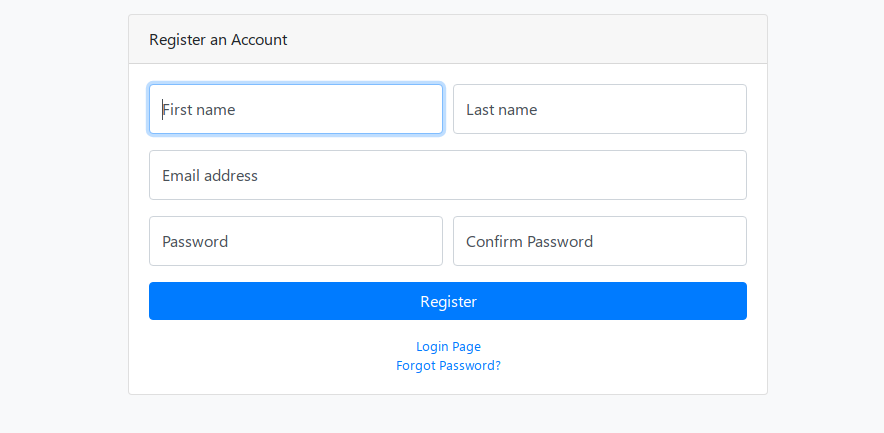
\includegraphics[width=0.85\linewidth]{figure/5-2}
	\caption{用户注册页面}
\end{figure}
\begin{figure}[H]
	\centering
	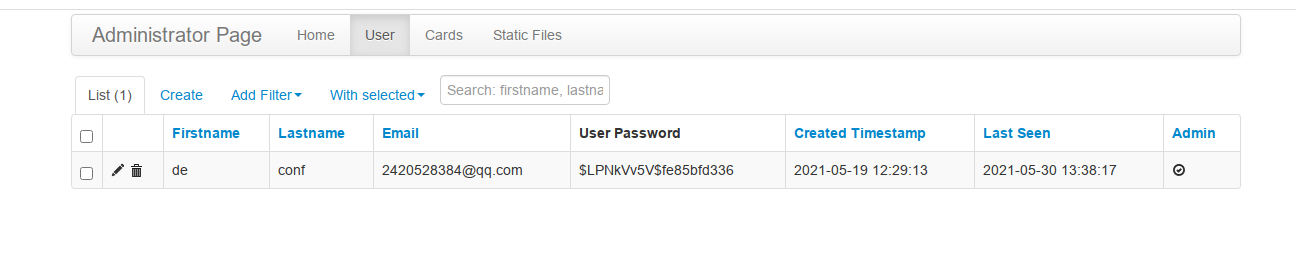
\includegraphics[width=0.85\linewidth]{figure/5-3}
	\caption{用户管理页面}
\end{figure}
\subsubsection{信息展示模块}
信息展示可以图形的方式直观的展示出节点的直观信息。方便直观的查看节点的环境参数,如当前的温度,湿度,烟雾等关键的环境信息,便于运维人员对于机房环境的监测。
\begin{figure}[H]
	\centering
	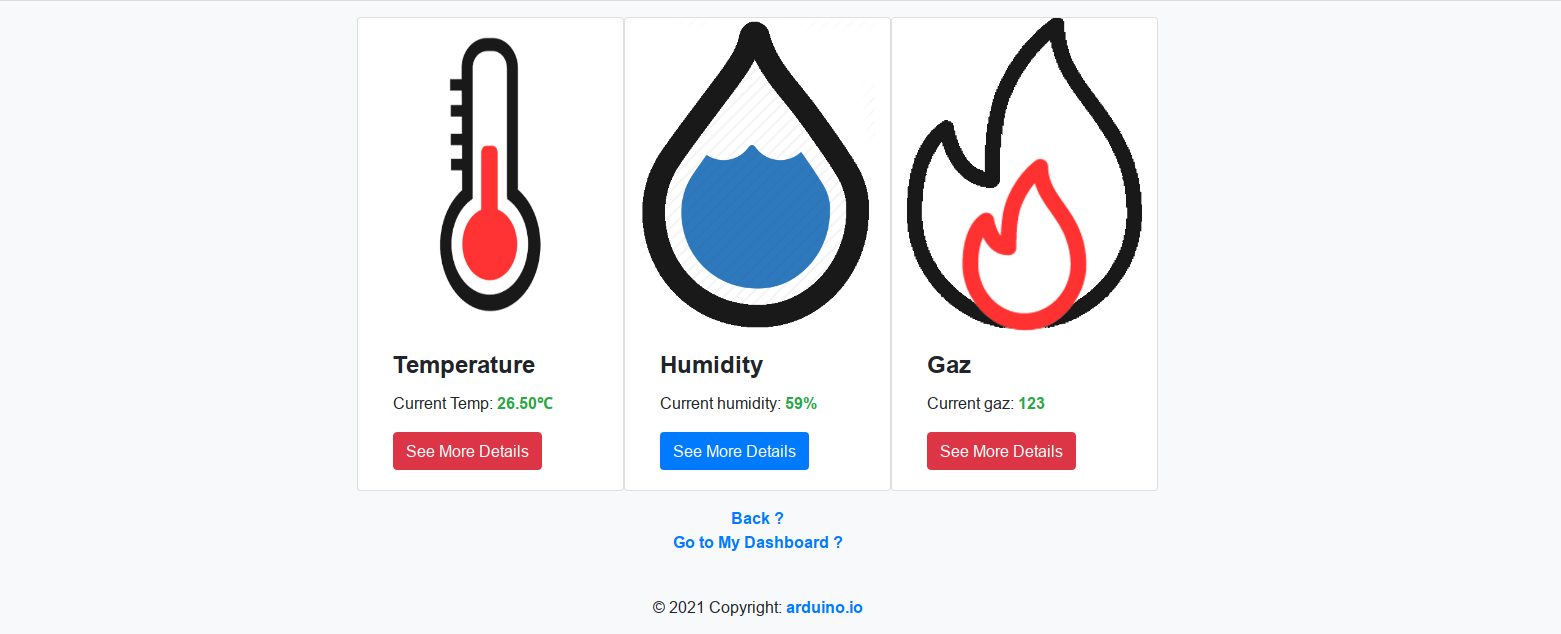
\includegraphics[width=0.85\linewidth]{figure/card_data}
	\caption{节点信息展示}
\end{figure}
\begin{figure}[H]
	\centering
	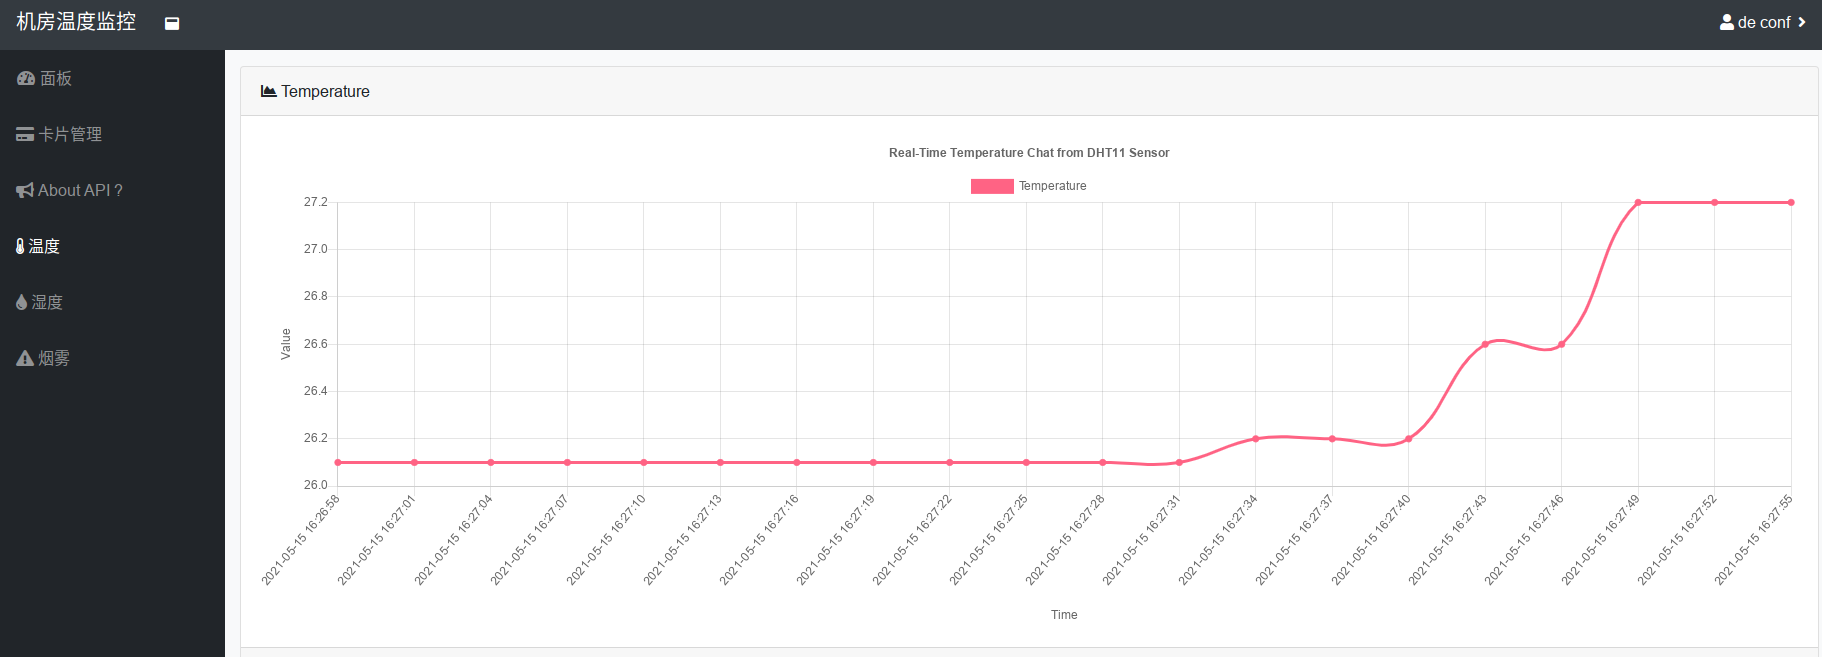
\includegraphics[width=0.85\linewidth]{figure/DHT11}
	\caption{温度显示模块}
\end{figure}
\begin{figure}[H]
	\centering
	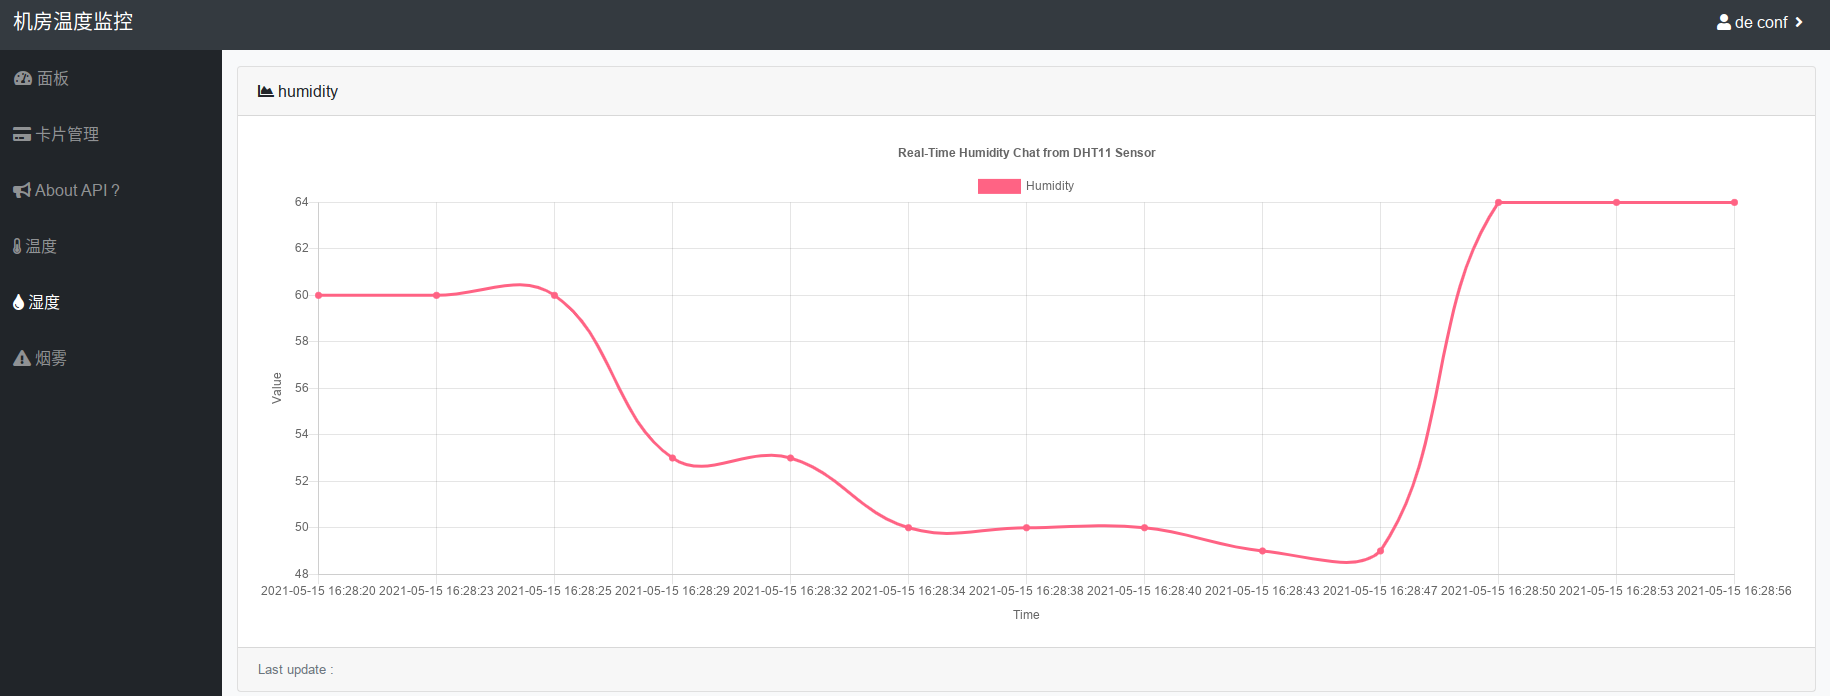
\includegraphics[width=0.85\linewidth]{figure/Humidity}
	\caption{湿度显示模块}
\end{figure}
\begin{figure}[H]
	\centering
	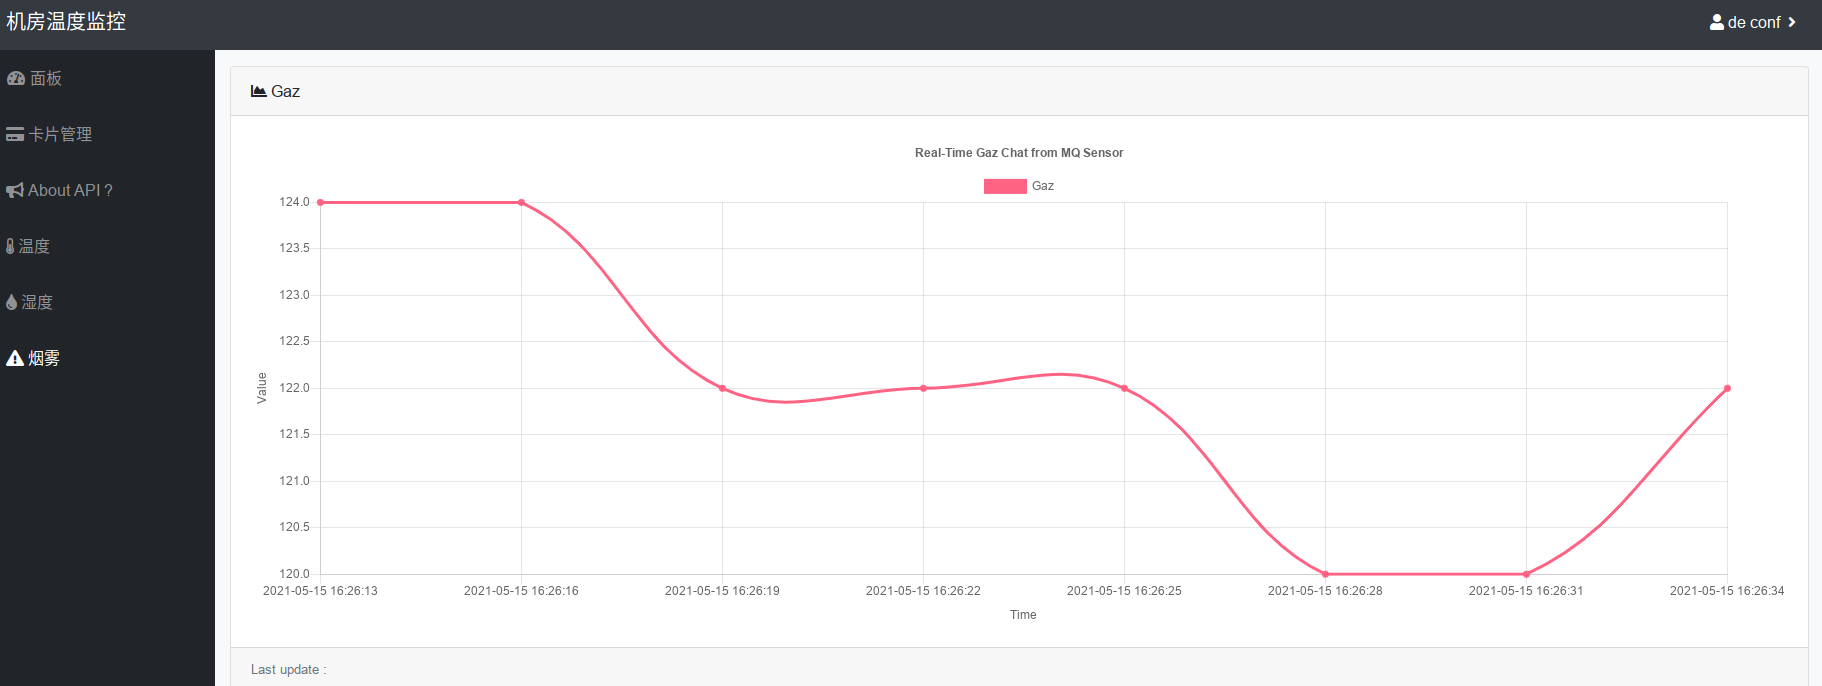
\includegraphics[width=0.85\linewidth]{figure/Gaz}
	\caption{烟雾显示模块}
\end{figure}

\subsubsection{节点管理模块}
通过这里可以方便快捷的对整个节点进行创建,删除。以及节点接受到数据的次数统计。通过次数统计可以对于客户端的传感器有鉴别,防止传感器因接线不良,传感器损坏导致的数据无法传输的问题。以及直观看到节点的API扩展信息。预留了数据整合的基础。
\begin{figure}[H]
	\centering
	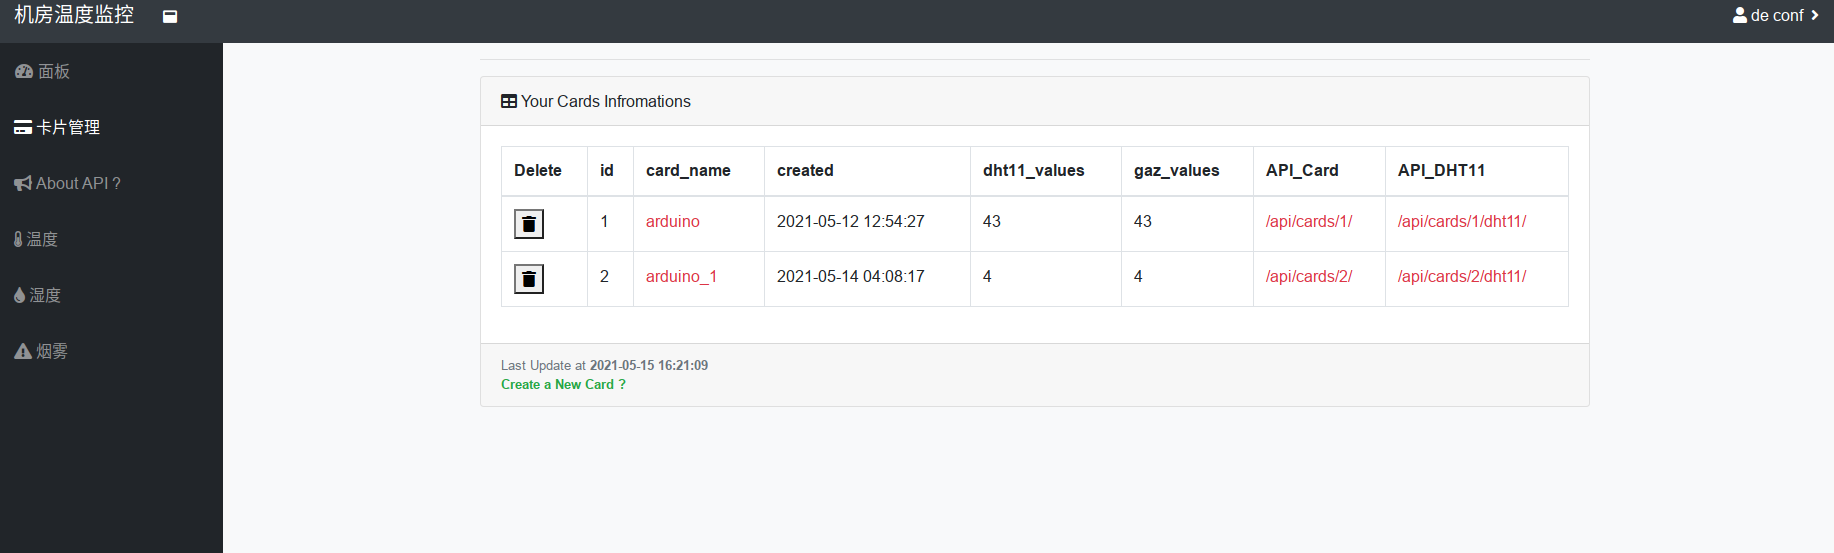
\includegraphics[width=0.85\linewidth]{figure/cards_edit}
	\caption{用户节点管理模块}
\end{figure}
\begin{figure}[H]
	\centering
	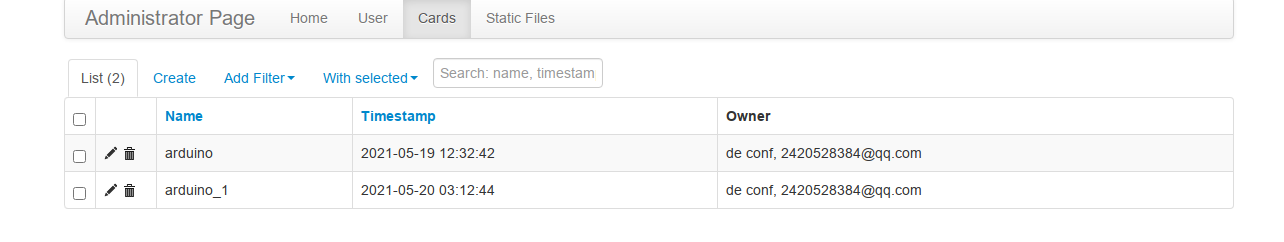
\includegraphics[width=0.85\linewidth]{figure/card_manage}
	\caption{管理员节点管理模块}
\end{figure}

\subsection{Arduino 客户端}

Arduino客户端主要负责节点环境信息采集,以及根据环境信息,控制空调。在各个传感器模块组装以及程序写入之后完成客户端的各项能力。通过DHT11温湿度传感器实现了环境温度、湿度信息采集,MQ2烟雾传感器模块实现了环境烟雾监测,并通过扩展的W5100以太网扩展模块向服务器传输节点的各项信息,如:温度,湿度,烟雾等环境信息。红外接收模块可以进行空调遥控器红外编码的解析,之后将解析后的数据保存在开发板内,可以通过开发板的红外发射模块,依照环境条件的阈值,进行相应的温湿度控制。

Arduino客户端的高扩展性和以及高开放性的特性在本次系统的起到了关键性作用。高扩展体现在Arduoino支持的多传感器设备,高开放性体现在代码中有各类对开源代码的复用。其设备的便捷性和可开发等特性带来了灵活便捷的组装或改装方式。例如,针对与WIFI联网环境可以替换W5100以太网模块为ESP8266模块即可完成WIFI下网络数据传输。在这些特性的支持下,Arduino的客户端具有了便捷的数据采集,传输方式。 

\begin{figure}[htbp]
	\centering
	\includegraphics[width=15cm, height=9cm]{figure/5-10}
	\caption{Arduino客户端展示图}
\end{figure}

\newpage
\subsection{遇到的问题和解决办法}
1. Arduino程序中断。具体表现为:只有串口连接后,程序才继续执行。
\\解决办法: 

阅读官方文档可知从Arduino IDE 1.0开始,串行传输是异步的。如果发送缓冲区中有足够的空白空间,Serial.write()则将在串行传输任何字符之前返回。如果发送缓冲区已满,Serial.write()则将阻塞直到缓冲区中有足够的空间。因此,为避免阻塞调用Serial.write(),需要注释掉程序中调试部分Serial.print()函数,防止引起IO阻塞。

2. Arduino开发板容量有限,无法存储空调设备的全部编码信息。
\\解决办法:

目前临时采用减少空调编码使用,减少空调的控制预设。在后期的优化中设想空调全部编码信息全部存储在服务器数据库中,之后通过MQTT协议进行下发,在通过数据拼接形成完整编码。

3. 红外发射后无反馈机制导致无法判定红外发射后空调是否相应以及生效。
\\解决办法:

通过增加声音感应模块确认空调接受的提示音。从而判断是否接受到Arduino红外控制信号。

	\section{系统测试}

系统测试是将需测试的软件,作为整个基于计算机系统的一个元素,与计算机硬件、外设、某些支持软件、数据和人员等其他系统元素及环境结合在一起测试。 在实际运行(使用)环境下,对计算机系统进行一系列的组装测试和确认测试。 系统测试的目的在于通过与系统的需求定义作比较,发现软件与系统定义不符合或与之矛盾的地方。

\subsection{测试目标}

\begin{enumerate}
	\item 查看系统中是否有逻辑错误以及逻辑冲突。发现系统中存在的问题,完善系统的设计逻辑。确保系统逻辑的稳定性,避免系统死锁等情况。
	\item 确立各个子模块以及主模块之间的状况。保证集成之后系统各模块之间的良好配合。
	\item 优化系统设计,找出系统缺陷,保证系统更加符合软件工程,可以得到良好的再维护可能。
	\item 进行实际的数据测试,保证各个模块能够对数据进行正常的数据处理和响应。
\end{enumerate}

\subsection{测试方案}

首先对于系统的各个子模块进行代码审查,如用户登录验证模块,节点管理模块等。确保各个子模块之间的代码的健壮性和稳健性。另外,还需要进行功能性测试,确保功能正常,可以按照预期目标产生相应的结果。

设计测试方案如下:
 
1. 通过MQTT客户端与服务端进行通信,查看服务端能否介绍到相应数据。测试过程如下所示:
\begin{figure}[htbp]
	\centering
	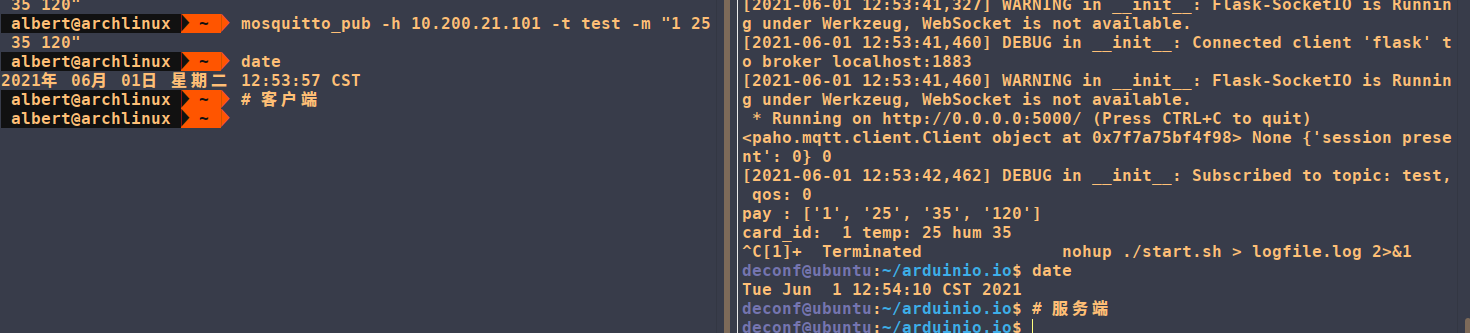
\includegraphics[width=0.85\linewidth]{figure/test-1}
	\caption{MQTT数据接受测试}
	\label{fig:6-1}
\end{figure}
如图\ref*{fig:6-1} 所示,MQTT服务器可以接收到相应的发送数据。

2. 检查MQTT服务器接收的数据是否存入到后端存储MySQL服务器中,测试过程如下所示:
\begin{figure}[htbp]
	\centering
	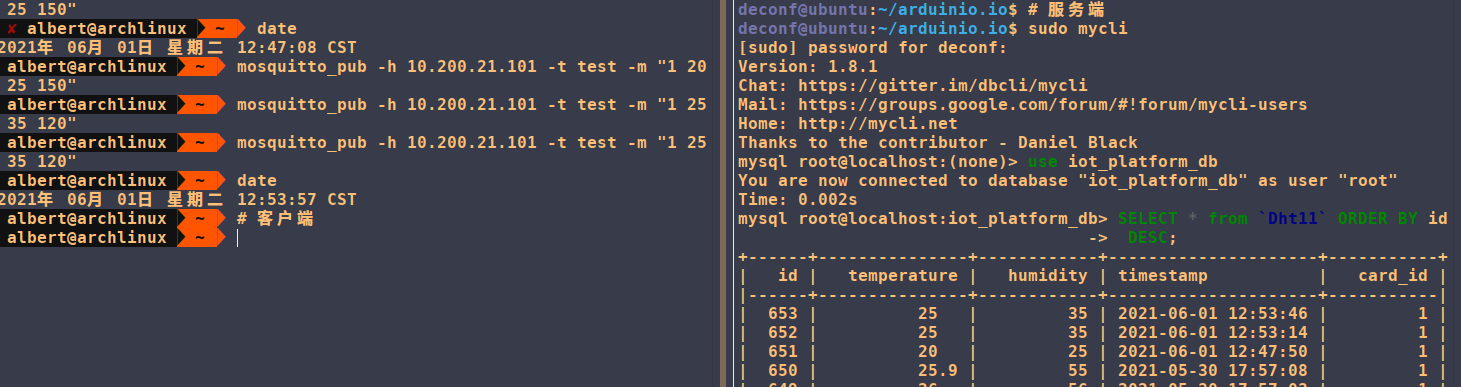
\includegraphics[width=0.85\linewidth]{figure/test-2}
	\caption{MQTT数据存储测试}
	\label{fig:6-2}
\end{figure}
如图\ref{fig:6-2} 通过时间戳可以判定数据已经接受并已经存储在后端MySQL服务器上。

3. 测试当数据超过设计相应的阈值,检查触发相应的警报模块,是否可以正常发送告警信息。
\begin{figure}[htbp]
	\centering
	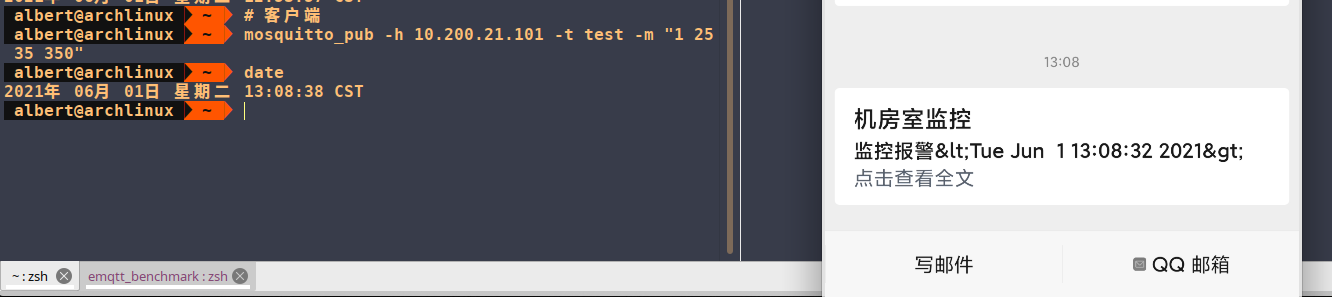
\includegraphics[width=0.85\linewidth]{figure/test-3}
	\caption{MQTT数据存储测试}
	\label{fig:6-3}
\end{figure}
如图\ref{fig:6-3}所示,在数据超过预设阈值之后,几乎可以同时收到相应的邮件告警信息。

\subsection{关于MQTT服务器高并发的测试}

\begin{table}[H]
	\centering
	\caption{测试环境配置}  %表格标题
	\begin{tabular}{ll} 
		\hline
		\hline
		核心硬件 & 型号 \\ 
		\hline
		CPU	& Intel Core i7 9xx (Nehalem Core i7, IBRS update) @ 6x 2.267GHz		\\
		RAM	& DDR3 1600MHz 4Gb \\
		HDD	& 40G \\
		\hline
		\hline
		核心软件 & 版本 \\ 
		\hline
		OS	& Ubuntu 18.04.5 LTS \\
		Python & v3.6.9 \\
		Flask & v1.0.3 \\
		mosquitto & v1.4.15 \\
		\hline
	\end{tabular}
\end{table}

此外,由于是分布式系统,那么对于系统的高并发测试也是必须进行的一个项目。服务器的高并发性能代表着服务器能容纳的节点数量以及可接入的客户端数量。代表之后可扩展的容量限制。

测试方案如下:

通过使用开源项目emqtt-bench模拟MQTT客户端与服务端进行通信,查看服务端的负载压力情况如下所示:


\begin{figure}[H]
	\centering
	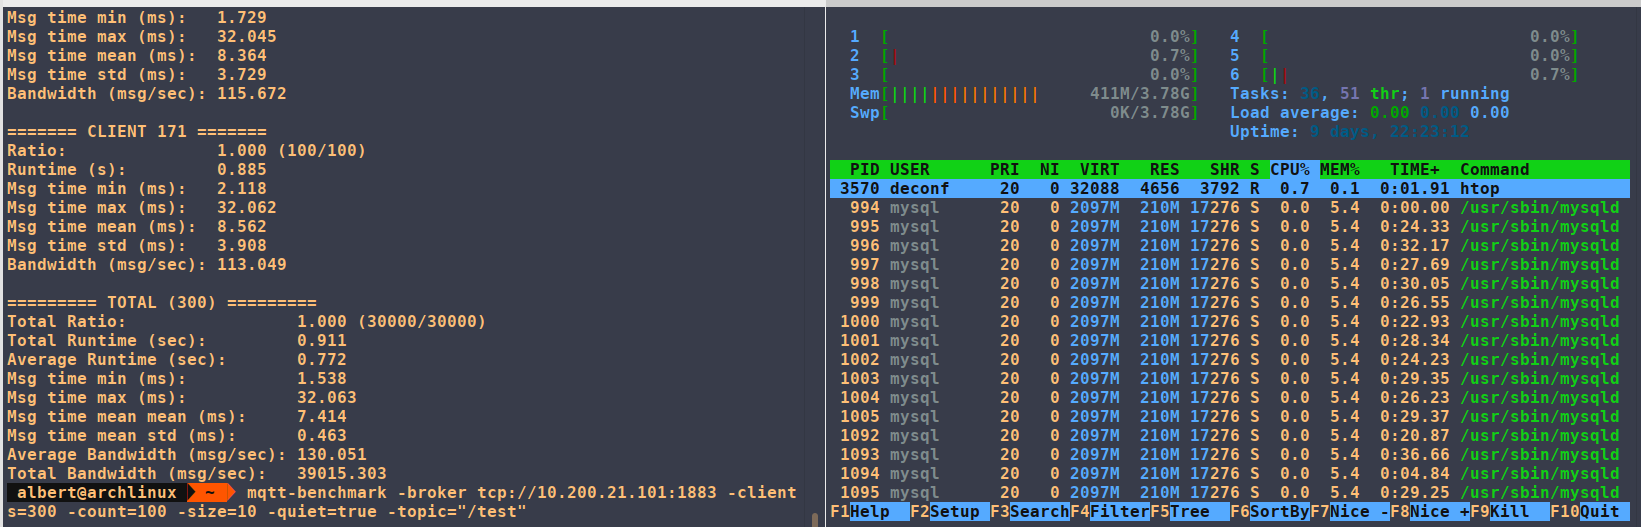
\includegraphics[width=0.85\linewidth]{figure/test-4}
	\caption{MQTT负载压力测试}
	\label{fig:6-4}
\end{figure}

如上图\ref{fig:6-4}在300个客户端同时订阅发布的情况下,得到了平均相应时间为0.772 ms
,最大响应时间为32.063ms,可以得出,系统可近似认为其为实时处理。
通过服务端的htop软件查看系统负债情况,发现MQTT服务端软件mosquitto几乎不占用负债情况。得益于MQTT协议的设计,在高并发的情况下,负载情况表现良好。
	% \fancypagestyle{summaryStyle}{
% 	\fancyhf{}
% 	\fancyhead[C]{\zihao{5} \songti 7\hspace{1em}结论与总结}
% }
% \thispagestyle{summaryStyle} 
\section{结论与总结}


依照基于Arduino的分布式温控系统的计划任务书的需求,首先进行系统的需求分析,之后进行整体设计,确定了Arduino客户端的程序流程和基于WEB温控系统的程序流程。论证了各项前沿的开发技术和开发方式,确定了整体项目框架以及数据库设计。采用了Arduino作为各节点信息采集的设备。其低廉的成本节省了大量的经费。Python的Flask作为开发WEB应用程序的框架,数据库采用了高效的MySQL。以及Linux作为操作系统。共同构成了完整的基于Arduino的分布式温度控制系统。

本系统基本完成了预期的目标:具有自动化的温度控制模块、远程可视化的环境温度、湿度、烟雾的监控模块,以及烟雾报警模块。基本满足了校园中通信机房智能化控制空调的能力。

本次系统开发离不开前期周密的技术调研,以及大量开源项目的使用。这些都很大程度的节省了开发代码的时间,并对该项目提供了很多方面的支持。

本次系统设计开发中,通过学习大量前沿项目经验,如ORM的数据库操控方式,RESTful的web架构,深入了解了最新的开发思想,开拓了编程思路。如ORM使得不必去书写复杂冗长的SQL命令语句,通过SQL的对象实例化,以编程的思路去控制数据库,这样减少不必要的数据库往返次数,增加了代码的一致性,提高了代码的复用性,使得编程效率有了很大的提高。



	
	%============= 参考文献 =====================
	\addcontentsline{toc}{section}{参考文献}
	\nocite{*}
	\bibliographystyle{gbt7714-2005}  % 论文引用格式
	\zihao{5} 
	\bibliography{bibfile}
	\zihao{-4} 
	
	%=============  致谢  ======================
	\fancypagestyle{acknowledge}{
    \fancyhf{}
	\fancyhead[C]{\zihao{5} \songti 西安石油大学大学本科毕业设计(论文)}
}
\thispagestyle{acknowledge}
\section*{致谢}
\addcontentsline{toc}{section}{致谢}

本次论文是在我的导师郑洪涛郑老师的悉心指导和亲切关心下完成的。他细心、认真地指导学生,提供了大量的设备支持以及理论探讨。从论文课题的筛选到最终项目的完成与上线投入运行,郑老师始终都给予了我细心指导和不懈支持。在此我向郑老师致以诚挚的谢意以及崇高的敬意。

另外,我还要感谢我的室友们解决问题的想法,以便我找到项目开发的最初方向。当然,他们也在业余时间,和我讨论关于算法的一些想法,让我受益匪浅。在这里,我说谢谢,希望这种友谊永远伴随着我。

在我上学十多年的过程中,离不开父母的鼓励和支持,是他们的辛勤工作、无私的付出,为我创造了良好的学习条件,让我可以完成学业,感激他们一直在养育我。

也许毕业设计是我在大学的最后一项作业。真的想借此机会给最近四年来帮助过我的所有老师、同学和朋友说声谢谢,你们的友谊将成为我一生最大的财富,是我人生不可分割的一部分。

在整个系统设计过程中,存在着许多障碍和挫折,但是当整个系统完全展现在自己面前时,这种喜悦溢于言表。近几个月忙于毕业设计,紧张而有条不紊,让我有机会对这个专业的基础理论、专业知识和基础技术有更深入的了解和体会,使我在大学里学到的知识体系升华。

这篇论文的撰写经验会让我牢记,并让我觉得我可以从头到尾地做一件事。它也教会了我细心做一件事的重要性。我希望这一经历能激励我继续在未来取得更多进步。

	
	%=============  附录 ======================
	%\include{body/appendices}
	
\end{document}
%%%%%%%%%% 结束 %%%%%%%%%%
